\chapter{Clock Generation}

\section{Introduction}

In the realm of computer architecture, the orchestration of tasks with meticulous precision is entrusted to the clock signal. At the heart of many computer systems lies a clock circuit, a symphony conductor orchestrating the synchronized movements of processors, memory, and peripherals. 

One prevalent method employed for generating these essential clock signals is the Pierce Oscillator, an elegantly designed circuit providing stability and accuracy.

\begin{theory}{Pierce Oscillator}
  The Pierce Oscillator, a popular choice in clock circuitry, utilizes the mechanical resonance of a quartz crystal to produce a stable and reliable clock signal. This oscillator configuration relies on a complementary metal-oxide-semiconductor (CMOS) inverter, a key amplifying element in the circuit.

  In operation, the quartz crystal resonator initiates oscillations by responding to an applied voltage, generating a consistent frequency as it vibrates. This crystal-induced frequency is then harnessed and refined by the CMOS inverter. The inverter, comprised of both PMOS and NMOS transistors, not only amplifies the signal but crucially introduces a 180-degree phase shift, laying the groundwork for sustained oscillations.

  The feedback loop, consisting of capacitors and resistors, ensures the necessary phase shifts to sustain oscillations, and the output is fine-tuned for accuracy. This marriage of the quartz crystal's stability and the CMOS inverter's amplification results in a clock signal that is both precise and dependable.
\end{theory}

In the realm of computer architecture, the use of the Pierce Oscillator for clock signal generation is a strategic choice. The stability provided by the quartz crystal, coupled with the amplifying capabilities of the CMOS inverter, ensures a reliable reference for synchronizing the myriad components within the system.

A well-designed Pierce Oscillator, integrated into the computer's motherboard or chip, becomes the heartbeat that regulates the flow of data, instructing processors when to execute operations and coordinating the harmonious collaboration of various subsystems. The meticulous design of this clock circuitry is paramount for the overall performance, reliability, and efficiency of modern computer systems.

In the subsequent sections, we will delve deeper into the intricacies of the Pierce Oscillator implemented in the Artemisa Computer System, examining its components, feedback mechanisms, and the role it plays in ensuring the precise orchestration of a computer's internal processes. Understanding these fundamentals is key to appreciating the inner workings of the clock circuitry that governs our digital machines.

\section{Circuit description}

The intricacies of the clock circuitry come to life in the circuit illustrated in Figure \ref{fig:artemisa-schematic-clock}. This circuit comprises two distinct yet interdependent sections. 

\begin{figure}[h]
  \centering
  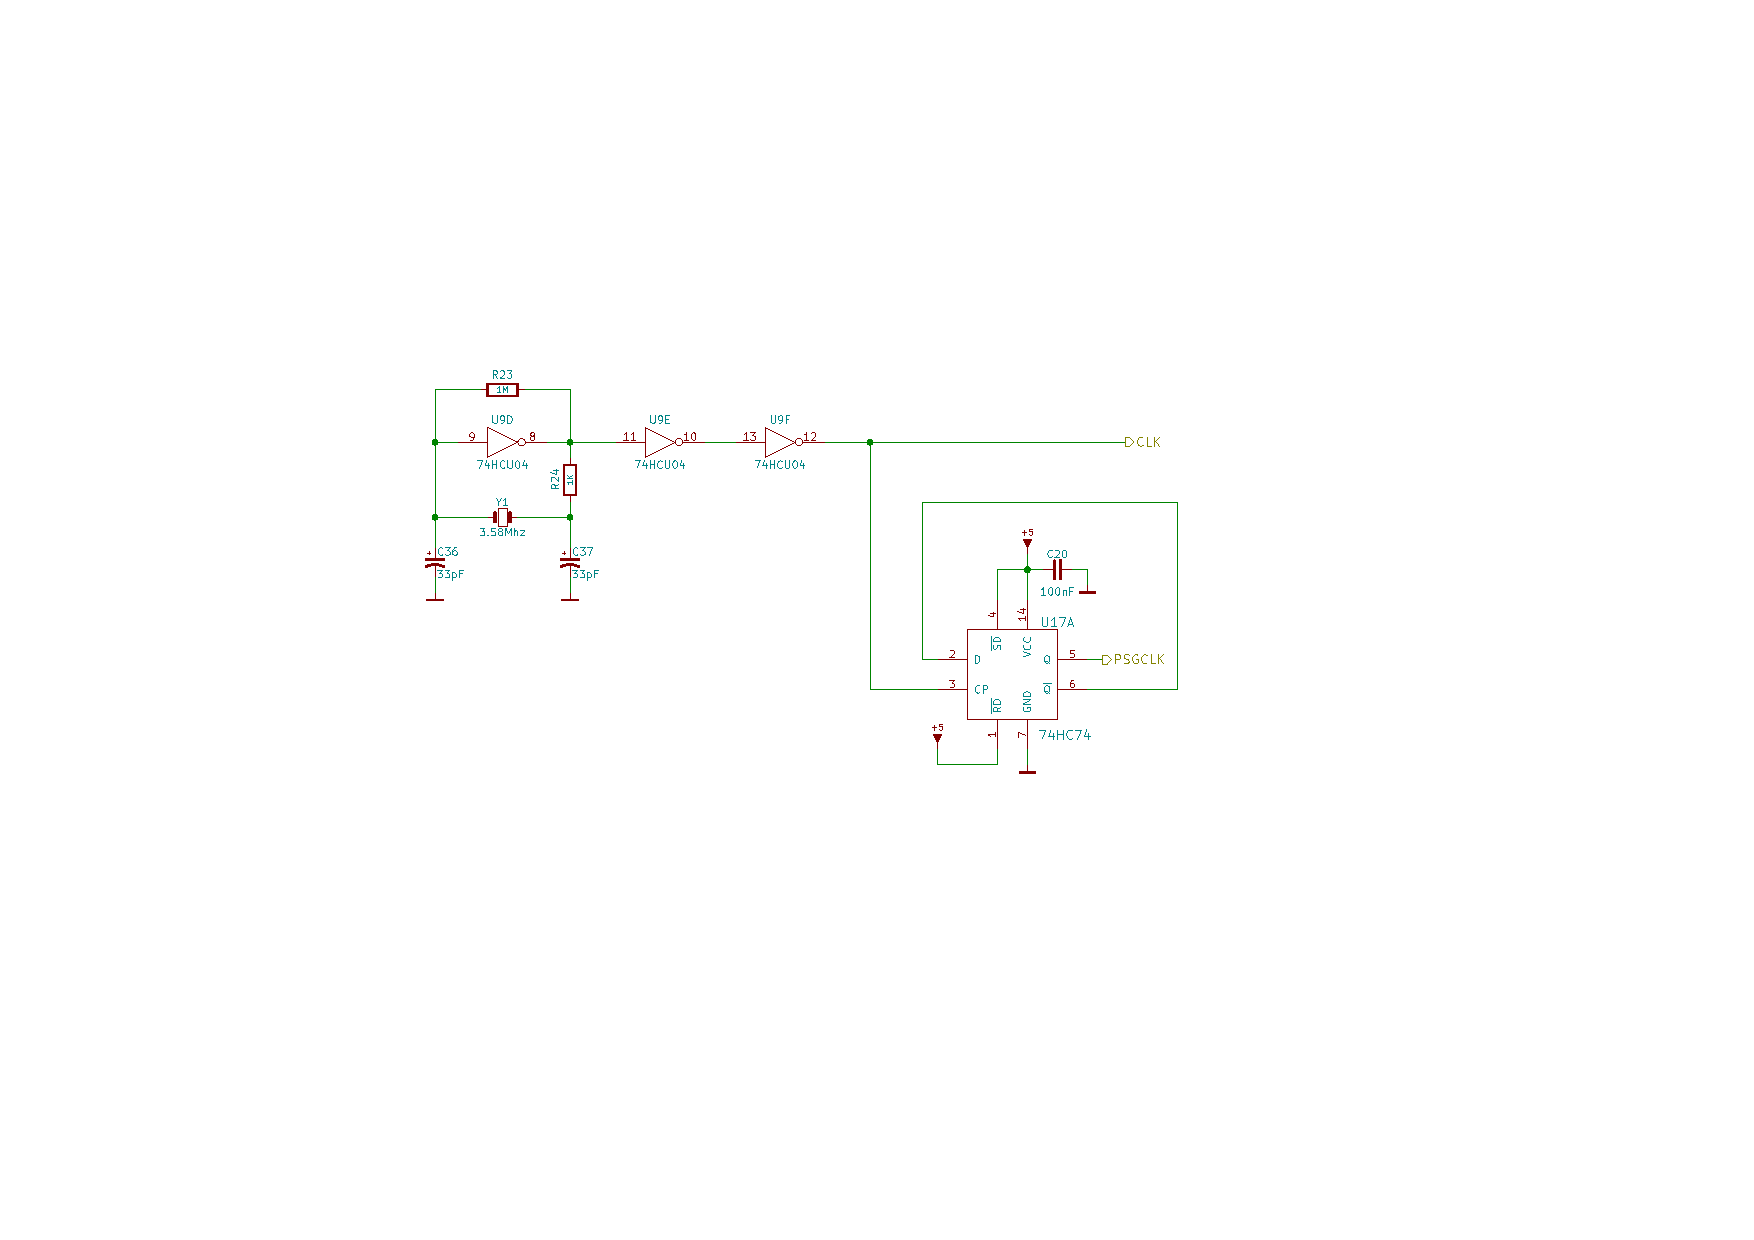
\includegraphics[width=\linewidth,trim={7cm 7.5cm 9cm 6cm},clip]{figures/artemisa-schematic-clock}
  \caption{Schematic diagram of clock generator}
  \label{fig:artemisa-schematic-clock}
\end{figure}

\begin{itemize}
  \item The first section on the left side of the figure unveils the elegant dance of the Pierce Oscillator, where the stable resonance of a quartz crystal, in tandem with the amplifying prowess of a CMOS inverter, forms the backbone of the system's clock signal. This section elucidates the foundational principles governing precise timekeeping and synchronization within the computer architecture. 
  \item The second section on the right side of the figure delves into the clock divider for the Programmable Sound Generator (PSG), showcasing how the rhythmic beats of the clock signal orchestrate the timing intricacies vital for sound synthesis. Together, these two sections represent the harmonious marriage of stability and division, ensuring the heartbeat of computing remains steady and resonant throughout the diverse symphony of a computer's operations.
\end{itemize}
  
\subsection{CPU clock from CMOS Pierce Oscillator}

Before delving into a detailed analysis of the clock circuit, it is prudent to first understand the fundamental principles of a basic oscillator. 

\begin{figure}[h]
  \centering
  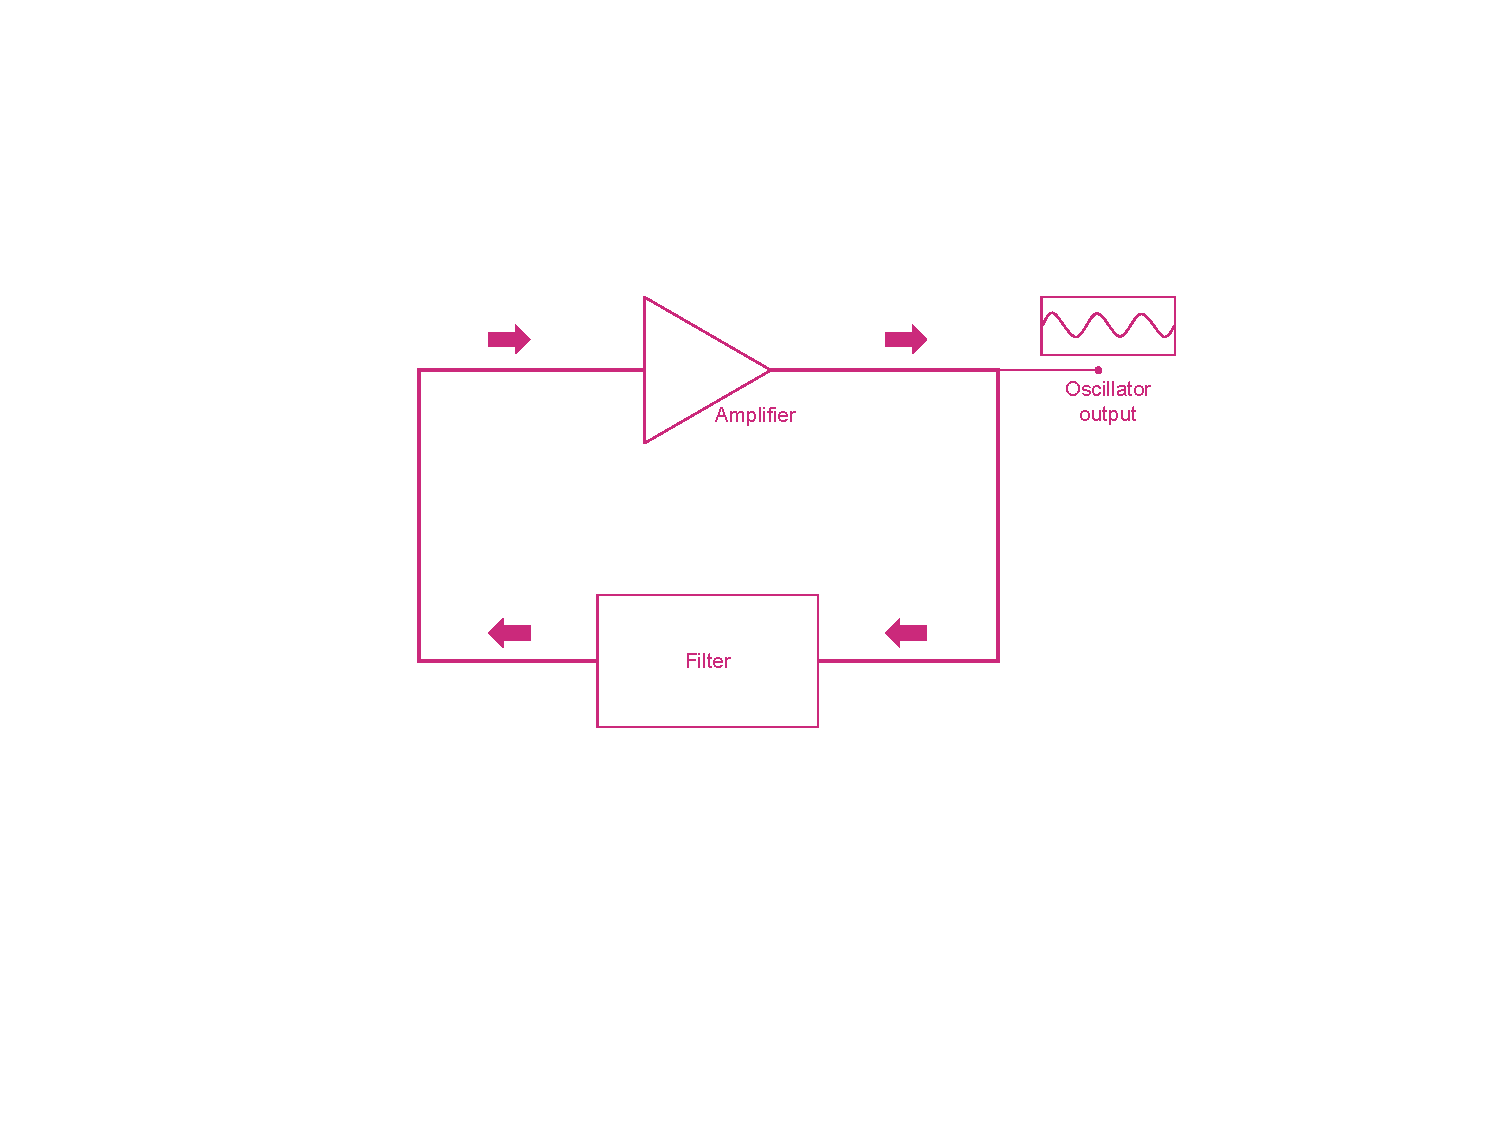
\includegraphics[width=\linewidth,trim={2cm 6cm 2cm 4cm},clip]{figures/oscillator-principle}
  \caption{Block diagram of a basic oscillator circuit}
  \label{fig:oscillator-principle}
\end{figure}

The most common form of linear oscillator is an electronic amplifier such as a transistor or operational amplifier connected in a feedback loop with its output fed back into its input through a frequency selective electronic filter to provide positive feedback, as shown in Figure \ref{fig:oscillator-principle}. 

In this configuration, the amplifier's output is directed back into its input through a frequency-selective electronic filter, creating a positive feedback loop. Upon the initial activation of the amplifier's power supply, electronic noise within the circuit initiates a non-zero signal, initializing oscillations. This inherent noise traverses the feedback loop, undergoing amplification and filtration processes, rapidly converging to generate a sinusoidal waveform at a specific frequency.

In order to work properly, this basic electronic oscillator must meet the {\bf Barkhausen Criteria}. Imagine you want to create a continuous sound in an electronic circuit, like a beep or a tone. The Barkhausen Criteria is like having the right setup to make sure that sound keeps going without fading away.

\begin{itemize}
  \item Amplification (Make it Loud): You need something to boost the sound signal, just like a speaker makes your music loud. This ensures the beep or tone doesn't die out.
  
  \item Positive Feedback (Keep the Vibe Going): Imagine clapping in a room, and the sound bounces back, creating a continuous applause. Positive feedback is like that: it sends a bit of the sound back to make sure the beep or tone doesn't stop.
  
  \item Phase Shift (Avoid the Noise): If your claps don't sync up, it becomes just noise. In electronics, phase shift makes sure the feedback sound aligns well with the original, so they work together, like a synchronized applause.
\end{itemize}
  
So, the Barkhausen Criteria is basically about making sure your electronic circuit has the right setup to keep a continuous sound, like a beep or a tone, going smoothly. More technically:

\begin{itemize}
  \item The product of the gains around the loop must be equal to or greater than one at the desired frequency of oscillation. In other words, the amplifier must provide a gain equal to or greater than one to sustain oscillations.
  \item The phase shift around the loop must be zero or any integer multiple of $2\pi$ (360º). In other words, the feedback network must provide the necessary phase shift to sustain oscillations.
\end{itemize}


\begin{figure}[h]
  \centering
  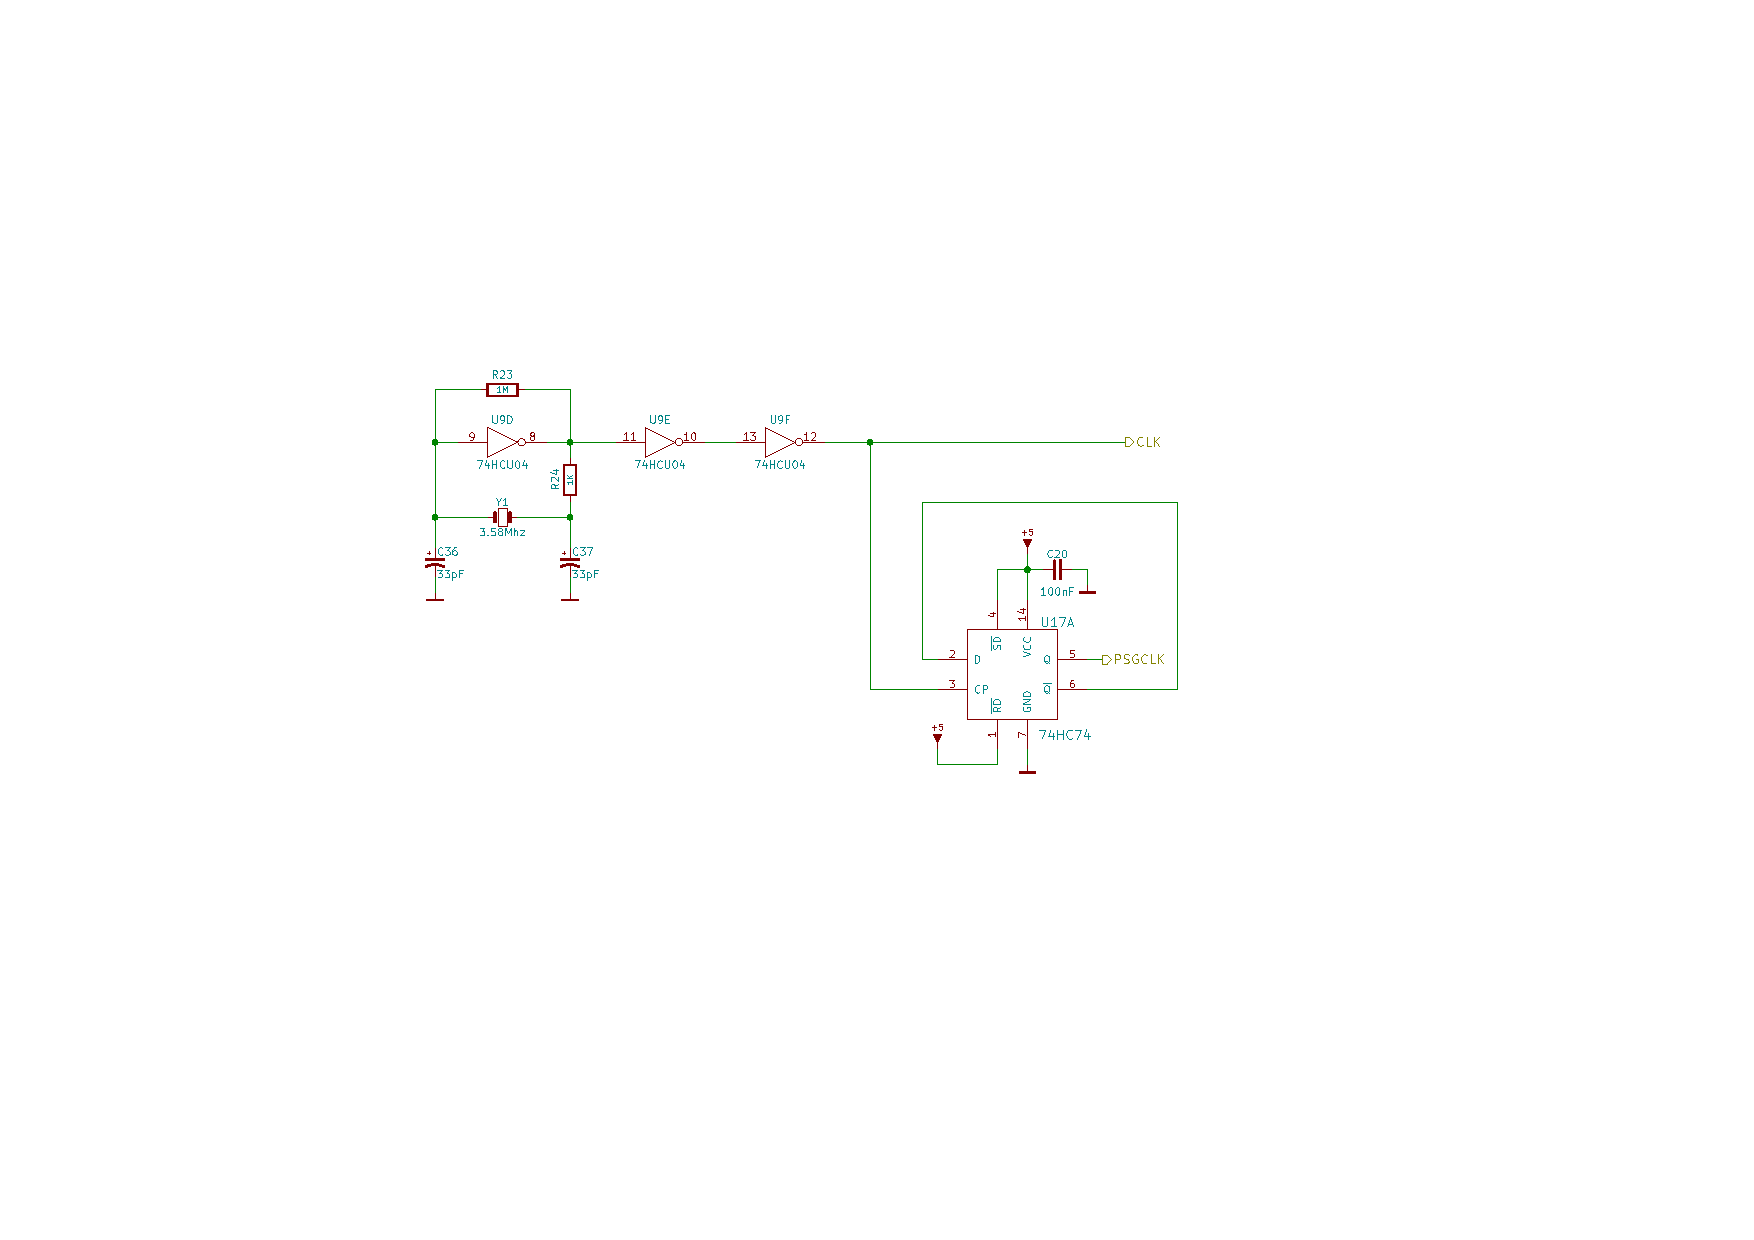
\includegraphics[width=.8\linewidth,trim={7cm 10.5cm 15.2cm 6cm},clip]{figures/artemisa-schematic-clock}
  \caption{Schematic diagram of CPU clock generation using a Pierce Oscillator circuit}
  \label{fig:artemisa-schematic-pierce-oscillator}
\end{figure}

In the context of a Pierce Oscillator utilizing a CMOS inverter, the fundamental elements of an oscillator are seamlessly integrated to produce a stable and precise clock signal, as shown in Figure \ref{fig:artemisa-schematic-pierce-oscillator}.

\begin{itemize}
  \item The CMOS inverter {\tt U9D} provides the necessary loop gain to sustain oscillation as well as approximately -180° phase shift. The part number of this inverter is {\tt 74JCU04}, where U means unbuffered. This is essential as the inverter must be able to operate as an amplifier in its linear region. The buffered inverters do not have this ability, and they would not produce a right amplification function.
  
  \item The feedback resistor {\tt R233} is there to linearize the digital CMOS inverter {\tt U9D}. It accomplishes this feat by charging the inverter's input capacitance, including {\tt C36} from the output of the inverter. In other words, the feedback resistor transforms a logic gate into an analog
  amplifier. Pretty neat trick by simply adding a single resistor.

  \item The resistor {\tt R24} in series with the output of the inverter is used to isolate the output driver of the inverter from the complex impedance formed by {tt C37}, {\tt C36} and the crystal {\tt Y1}. Without this resistor, the output of the inverter could physically damage the crystal.
  
  \item The crystal {\tt Y1}, together with {\tt C36}, {\tt C37} and {\tt R24}, provide an additional -180° phase lag to satisfy the Barkhausen phase shift criteria for sustaining oscillation. The crystal needs to be a {\it Parallel Mode}, {\it Fundamental} crystal.
  
  \item The inverters {\tt U9E} and {\tt U9F} are used to buffer the clock signal, generating a squared waveform with a 50\% duty cycle that can drive the CPU clock input.
\end{itemize}

\subsection{PSG clock from CPU clock divider}

\begin{figure}[h]
  \centering
  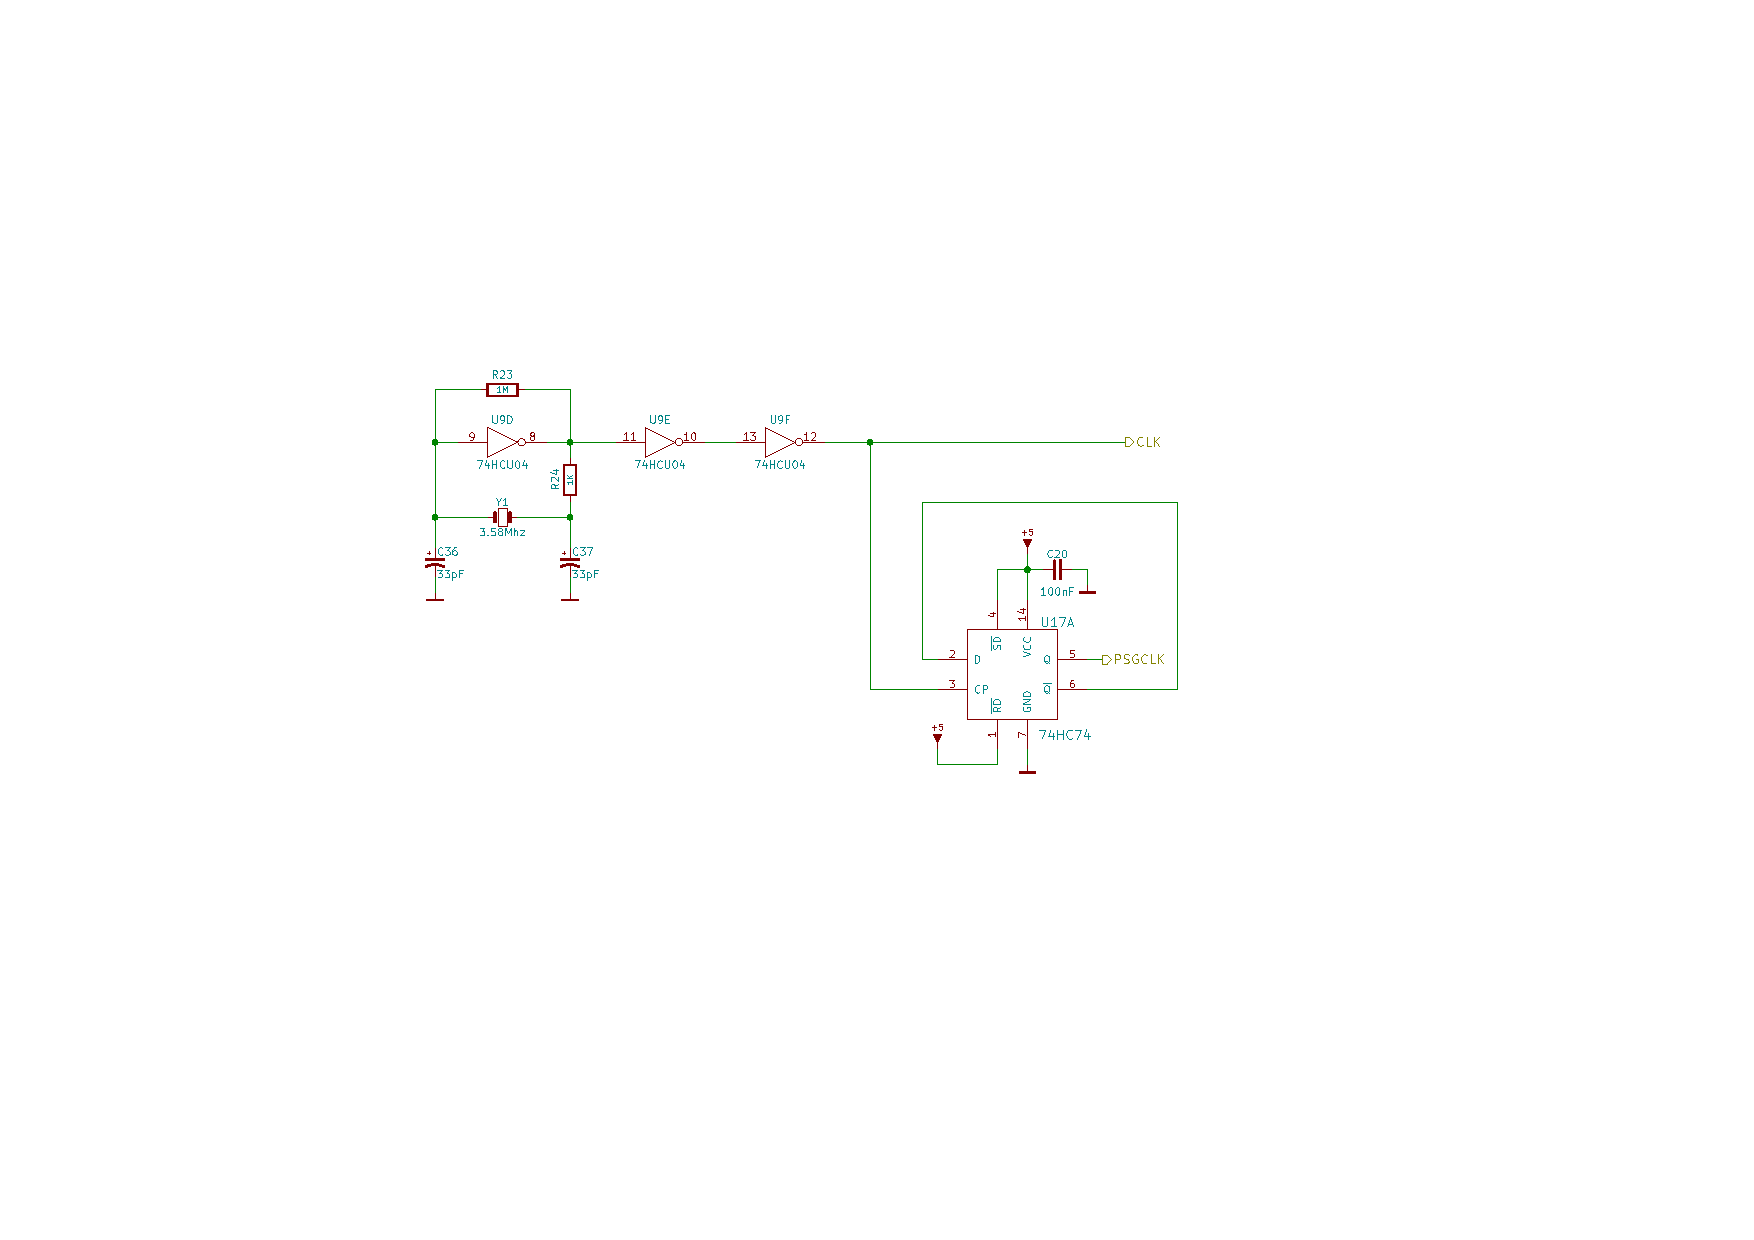
\includegraphics[width=.6\linewidth,trim={14cm 7.5cm 9cm 7cm},clip]{figures/artemisa-schematic-clock}
  \caption{Schematic diagram of PSG clock divider}
  \label{fig:artemisa-schematic-psg-clock}
\end{figure}

The Programmable Sound Generator (PSG) is a sound chip that provides three square wave tone generators and one noise generator. These generators depend on a periodic clock signal to produce the output waveforms. 

The PSG used by Artemisa is the General Instrument AY-3-8910. This device requires a clock input frequency between 1Mhz and 2Mhz. The clock's frequency determines the output tone frequency. The MSX system is designed to make this device operate at 1.79Mhz, which is half the frequency of the CPU clock.

Hence, in order to produce a valid PSG clock signal all we have to do is to divide the CPU clock by two. This is accomplished by the clock divider circuit shown in Figure \ref{fig:artemisa-schematic-psg-clock}.

\begin{figure}[h]
  \centering
  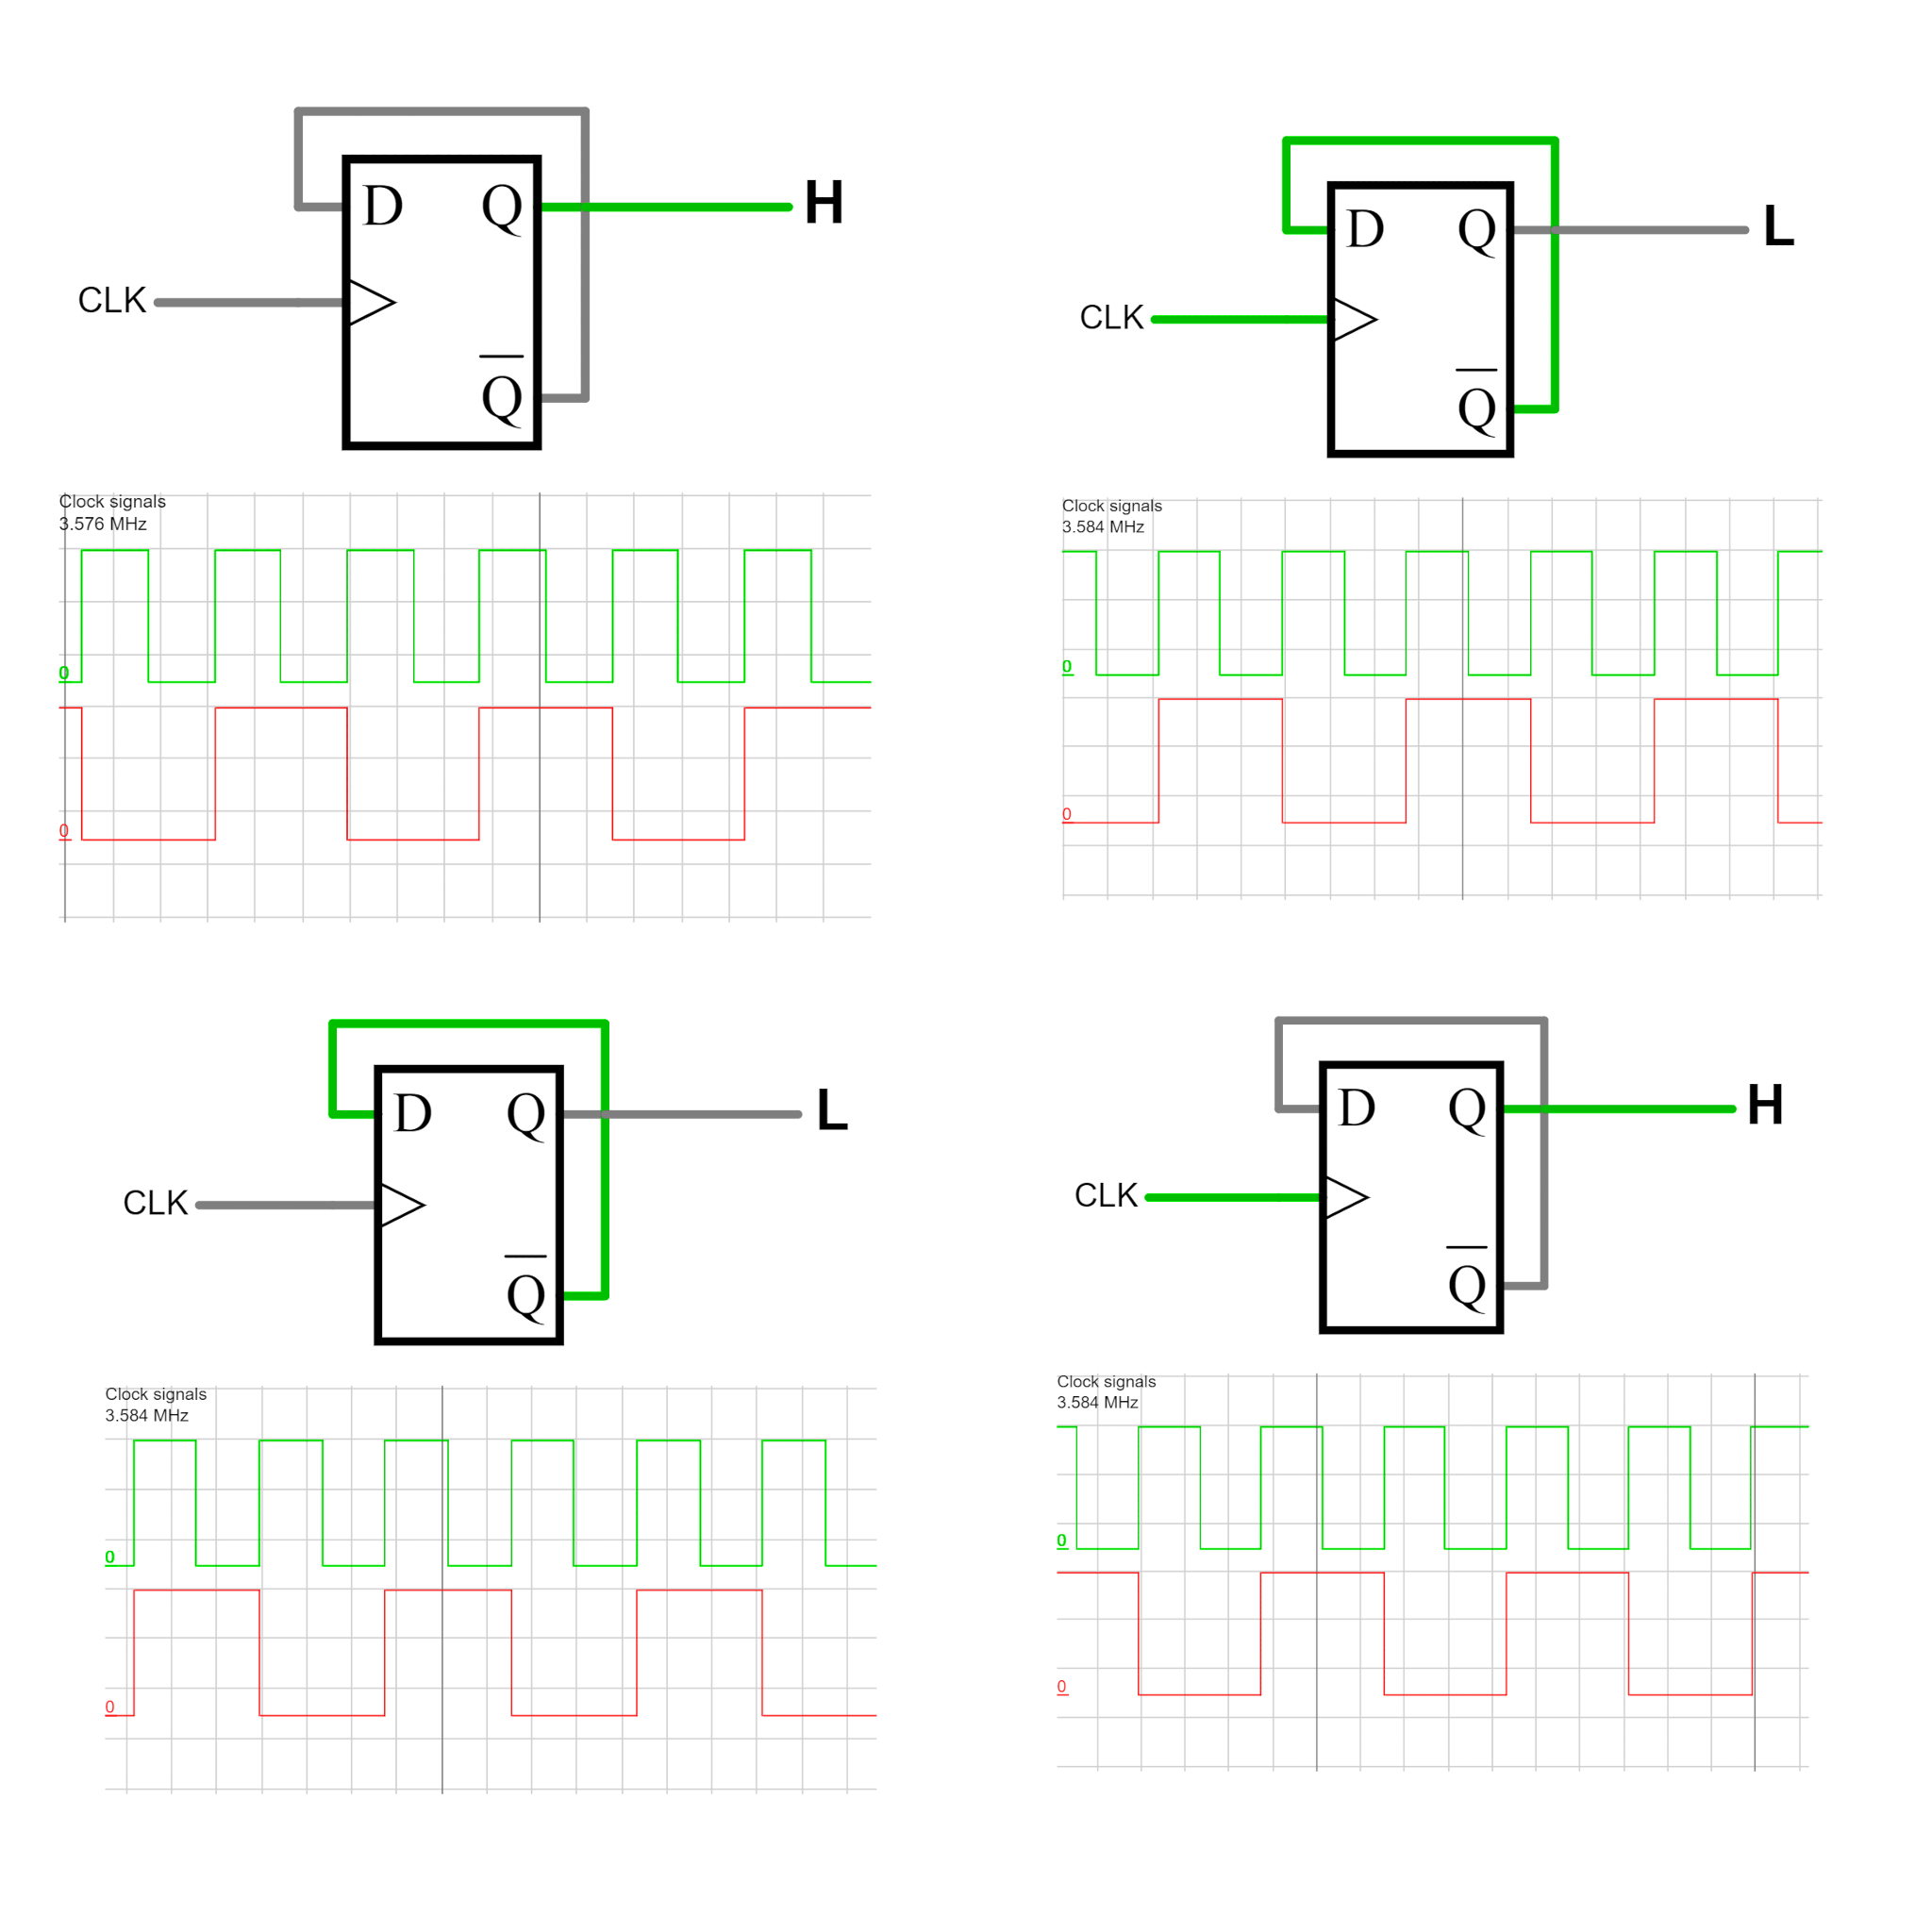
\includegraphics[width=.8\linewidth,trim={0cm 0cm 0cm 0cm},clip]{figures/simul-psg-clock}
  \caption{Simulation of the PSG clock divider circuit}
  \label{fig:simul-psg-clock}
\end{figure}

\begin{theory}{D-Type Flip-Flop}
  A D-type flip-flop is a basic digital circuit with two main inputs: the Data (D) input and the Clock (Clk) input. Its primary output is denoted as Q.
  
  The operation of a D-type flip-flop is triggered by changes in the clock signal. When the clock transitions (from low to high or high to low), the flip-flop captures the data present at the D input and transfers it to the Q output. If D is high during the clock transition, Q becomes high, and if D is low, Q becomes low. The flip-flop essentially acts as a memory element, retaining its output state until the next clock transition. 
  
  Some D-type flip-flops may include additional features like clock enable (EN) or asynchronous clear (CLR) and preset (PR) inputs. EN allows the flip-flop to ignore clock transitions when low, and CLR/PR inputs force the Q output to a defined state when activated. D-type flip-flops find widespread use in sequential logic and memory applications, forming the basis for various digital systems.  
\end{theory}

The circuit is comprised of a D-type flip-flop {\tt U17A}. The {\tt CP} input of the flip-flop is connected to the CPU clock signal, and the {\tt D} input is connected to the {\tt /Q} output of the flip-flop. On each rising edge of the CPU clock, the flip-flop stores the value of the {\tt /Q} output, which is the reverse value that was stored in the previous CPU cycle. As {\tt /Q} is used to feed the {\tt D} input instead of {\tt Q}, the flip-flop will toggle its output on each rising edge of the CPU clock, generating a clock signal with half the frequency of the CPU clock, as shown in the simulation in Figure \ref{fig:simul-psg-clock}. The {\tt Q} output of the flip-flop is the PSG clock signal.

The {\tt /SD} and {\tt /RD} signals of the 74HC74 flip-flop are used to set and reset, respectively, the stored value. In this particular case, it is not necessary to set or reset the flip-flop on any time, so these signals are tied to 5V to be inactive.

\section{Circuit assembly}

\subsection{Crystal oscillator circuit}

We will start by assembling the elements of the crystal oscillator circuit described in Figure \ref{fig:artemisa-schematic-pierce-oscillator}: 

\begin{enumerate}
  \item Solder the resistors {\tt R23} and {\tt R24}, whose placement is shown in Figure \ref{fig:mount-clock-cpu-01}.
  \item Solder the ceramic capacitors {\tt C36} and {\tt C37}, whose placement is shown in Figure \ref{fig:mount-clock-cpu-02}.
  \item Solder the quartz crystal {\tt Y1}, whose placement is shown in Figure \ref{fig:mount-clock-cpu-03}.
  \item Solder the CMOS inverter 74HCU04 {\tt U9}, whose placement is shown in Figure \ref{fig:mount-clock-cpu-04}.
\end{enumerate}


\begin{figure}[htbp]
  \centering
  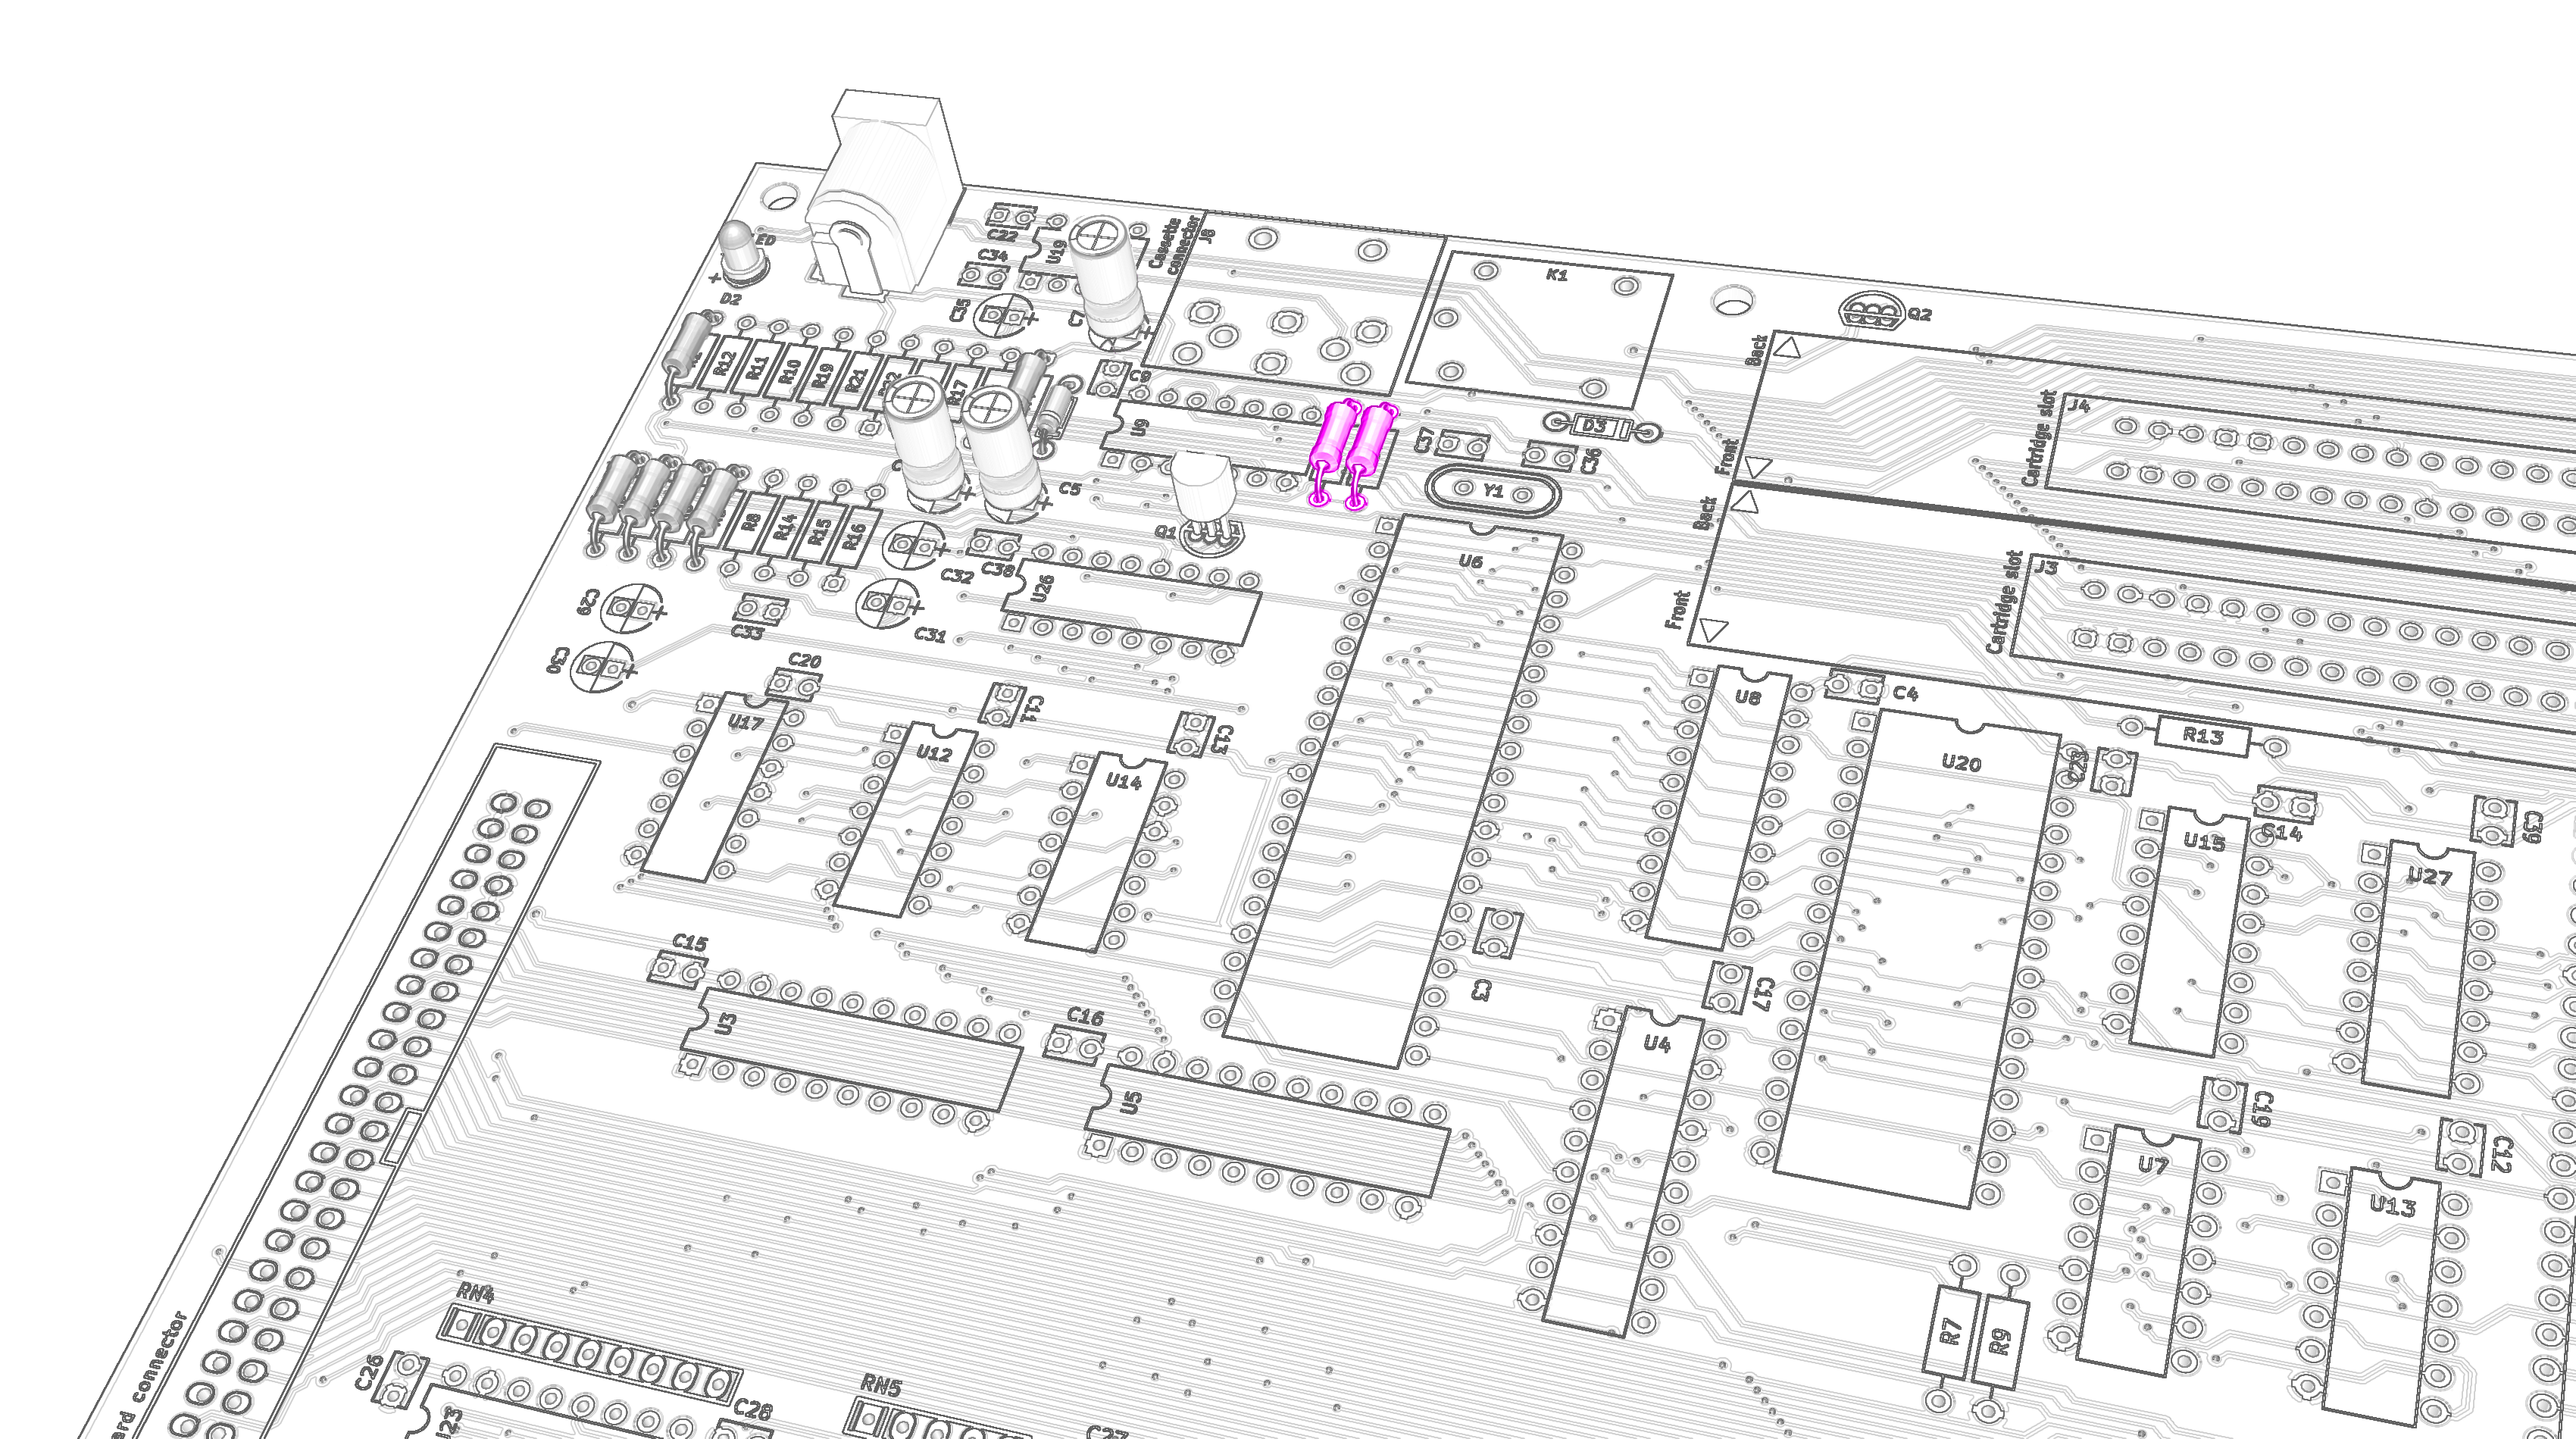
\includegraphics[width=0.8\linewidth]{figures/mount-clock-cpu-01}
  \caption{Placement of resistors {\tt R23} and {\tt R24} of the CPU clock generator}
  \label{fig:mount-clock-cpu-01}
\end{figure}

\begin{figure}[htbp]
  \centering
  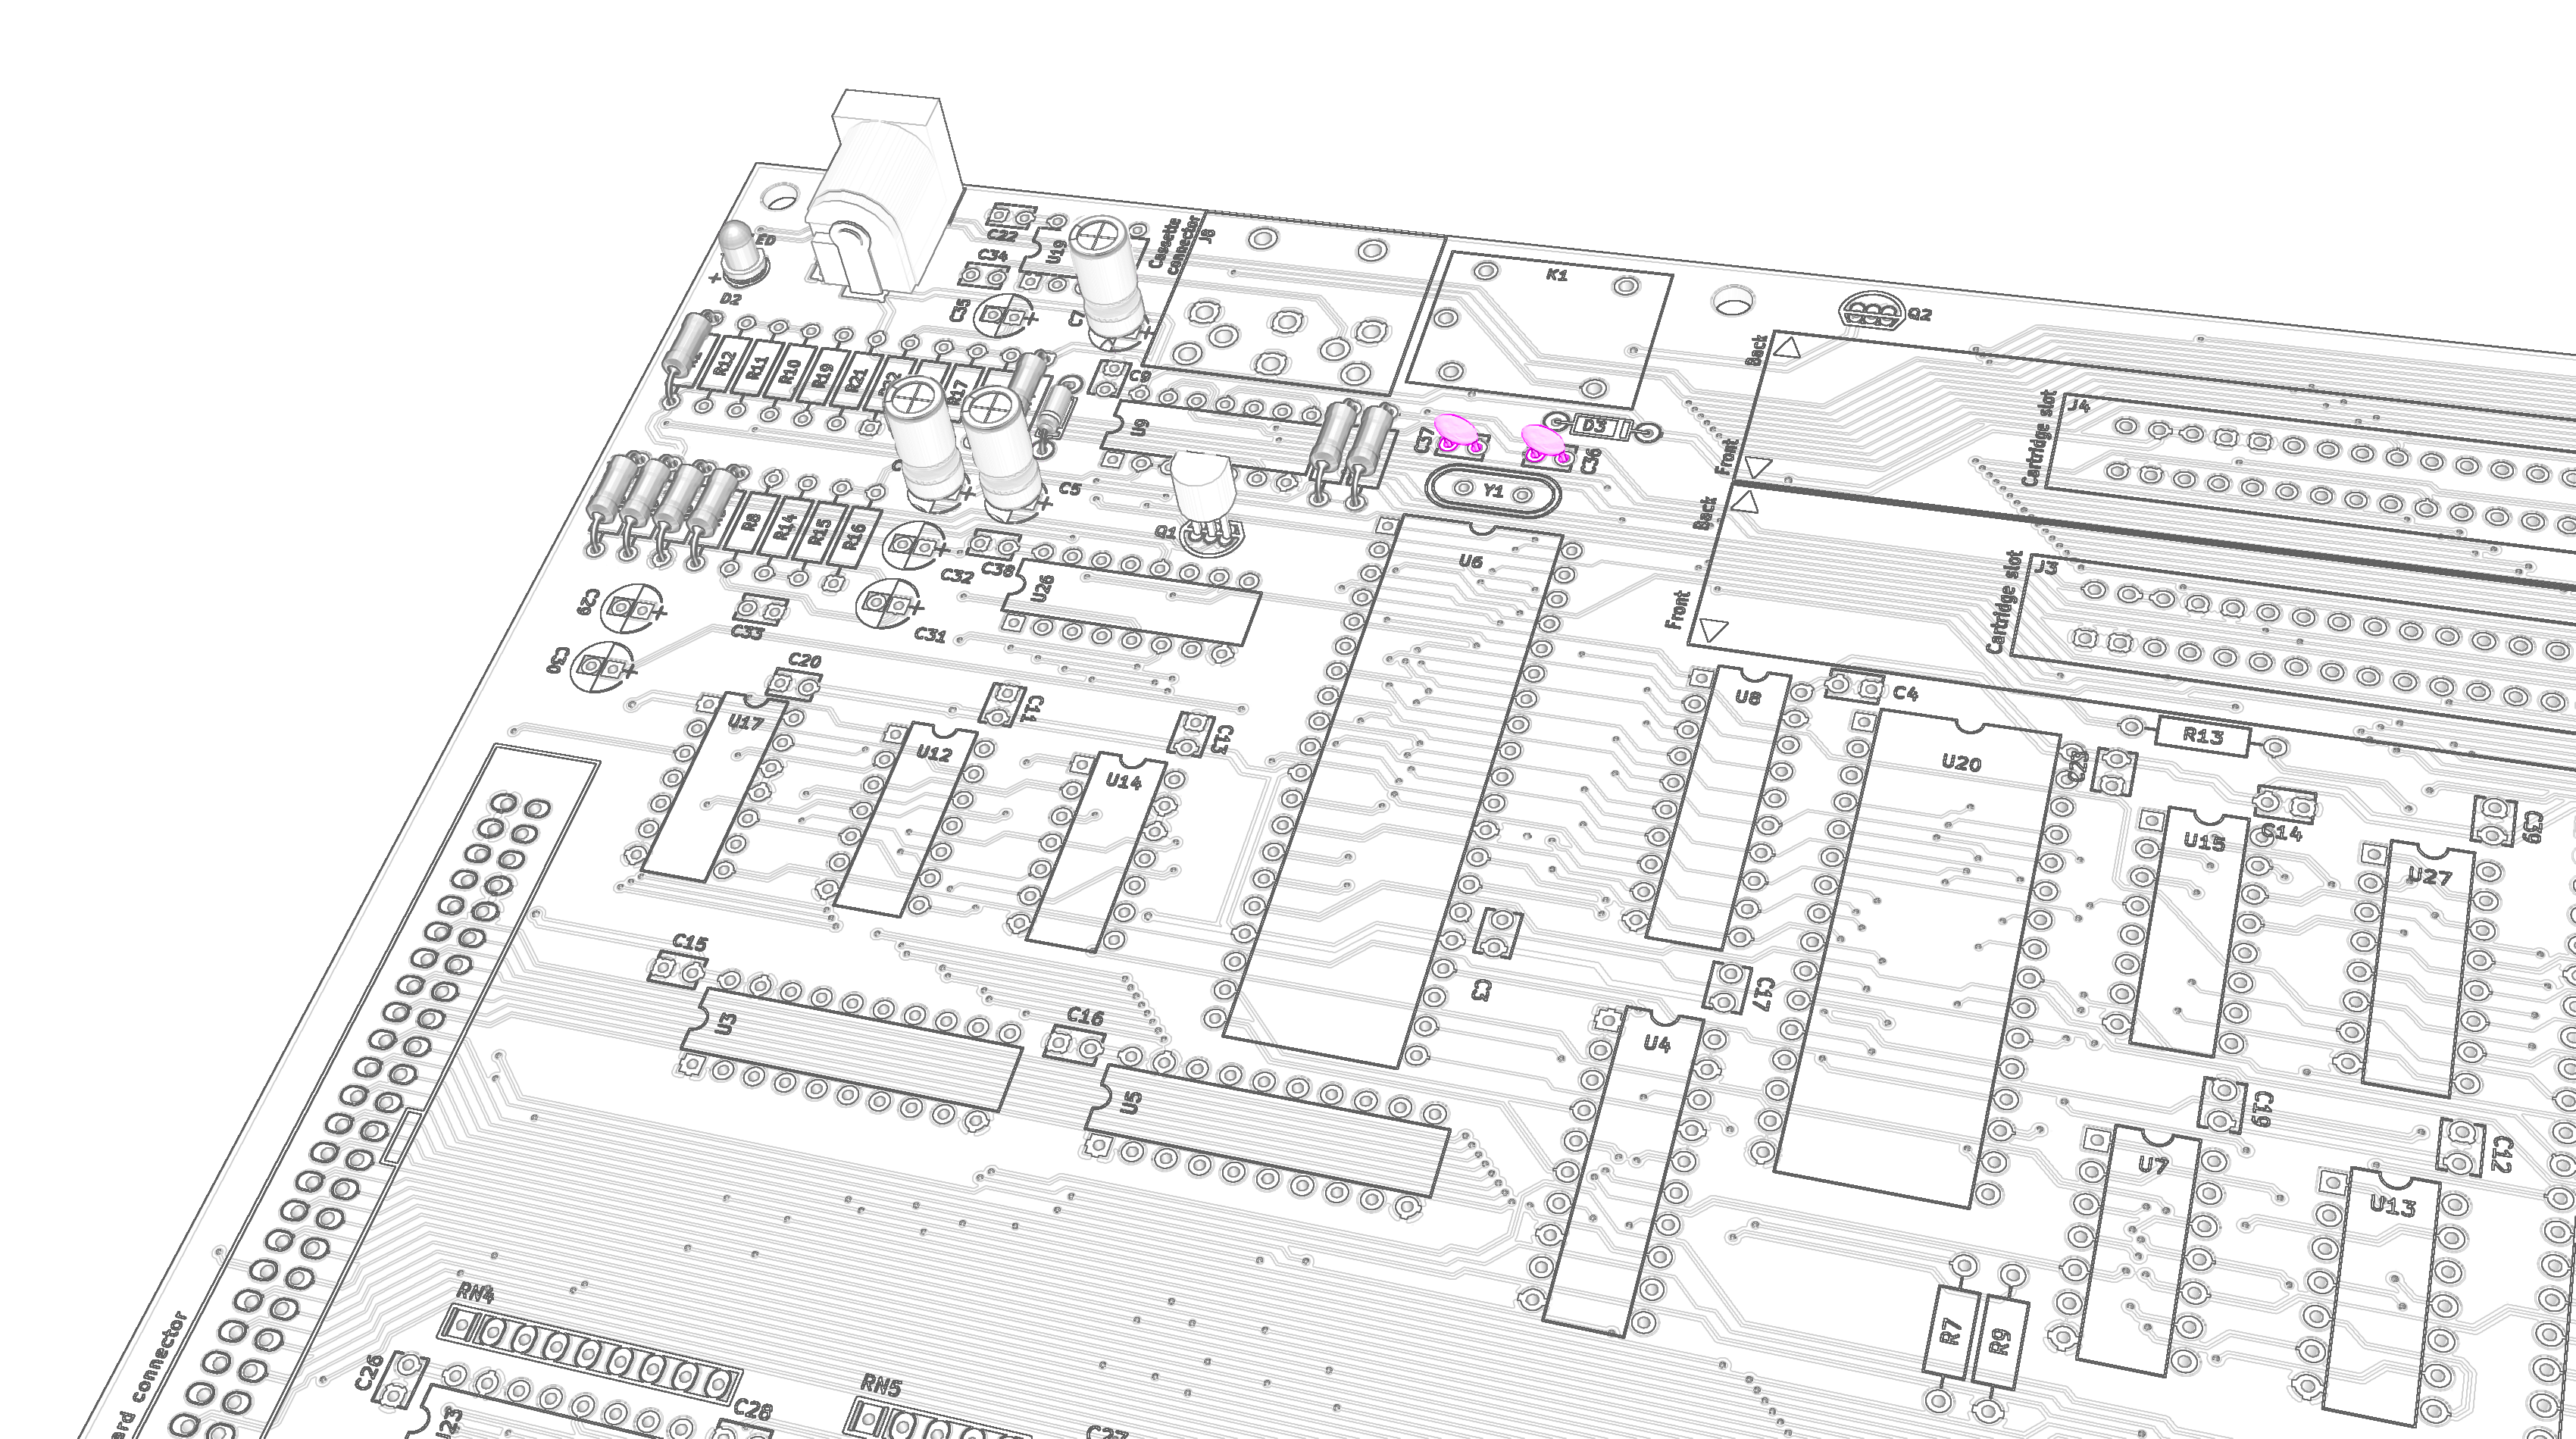
\includegraphics[width=0.8\linewidth]{figures/mount-clock-cpu-02}
  \caption{Placement of capacitors {\tt C36} and {\tt C37} of the CPU clock generator}
  \label{fig:mount-clock-cpu-02}
\end{figure}

\begin{figure}[htbp]
  \centering
  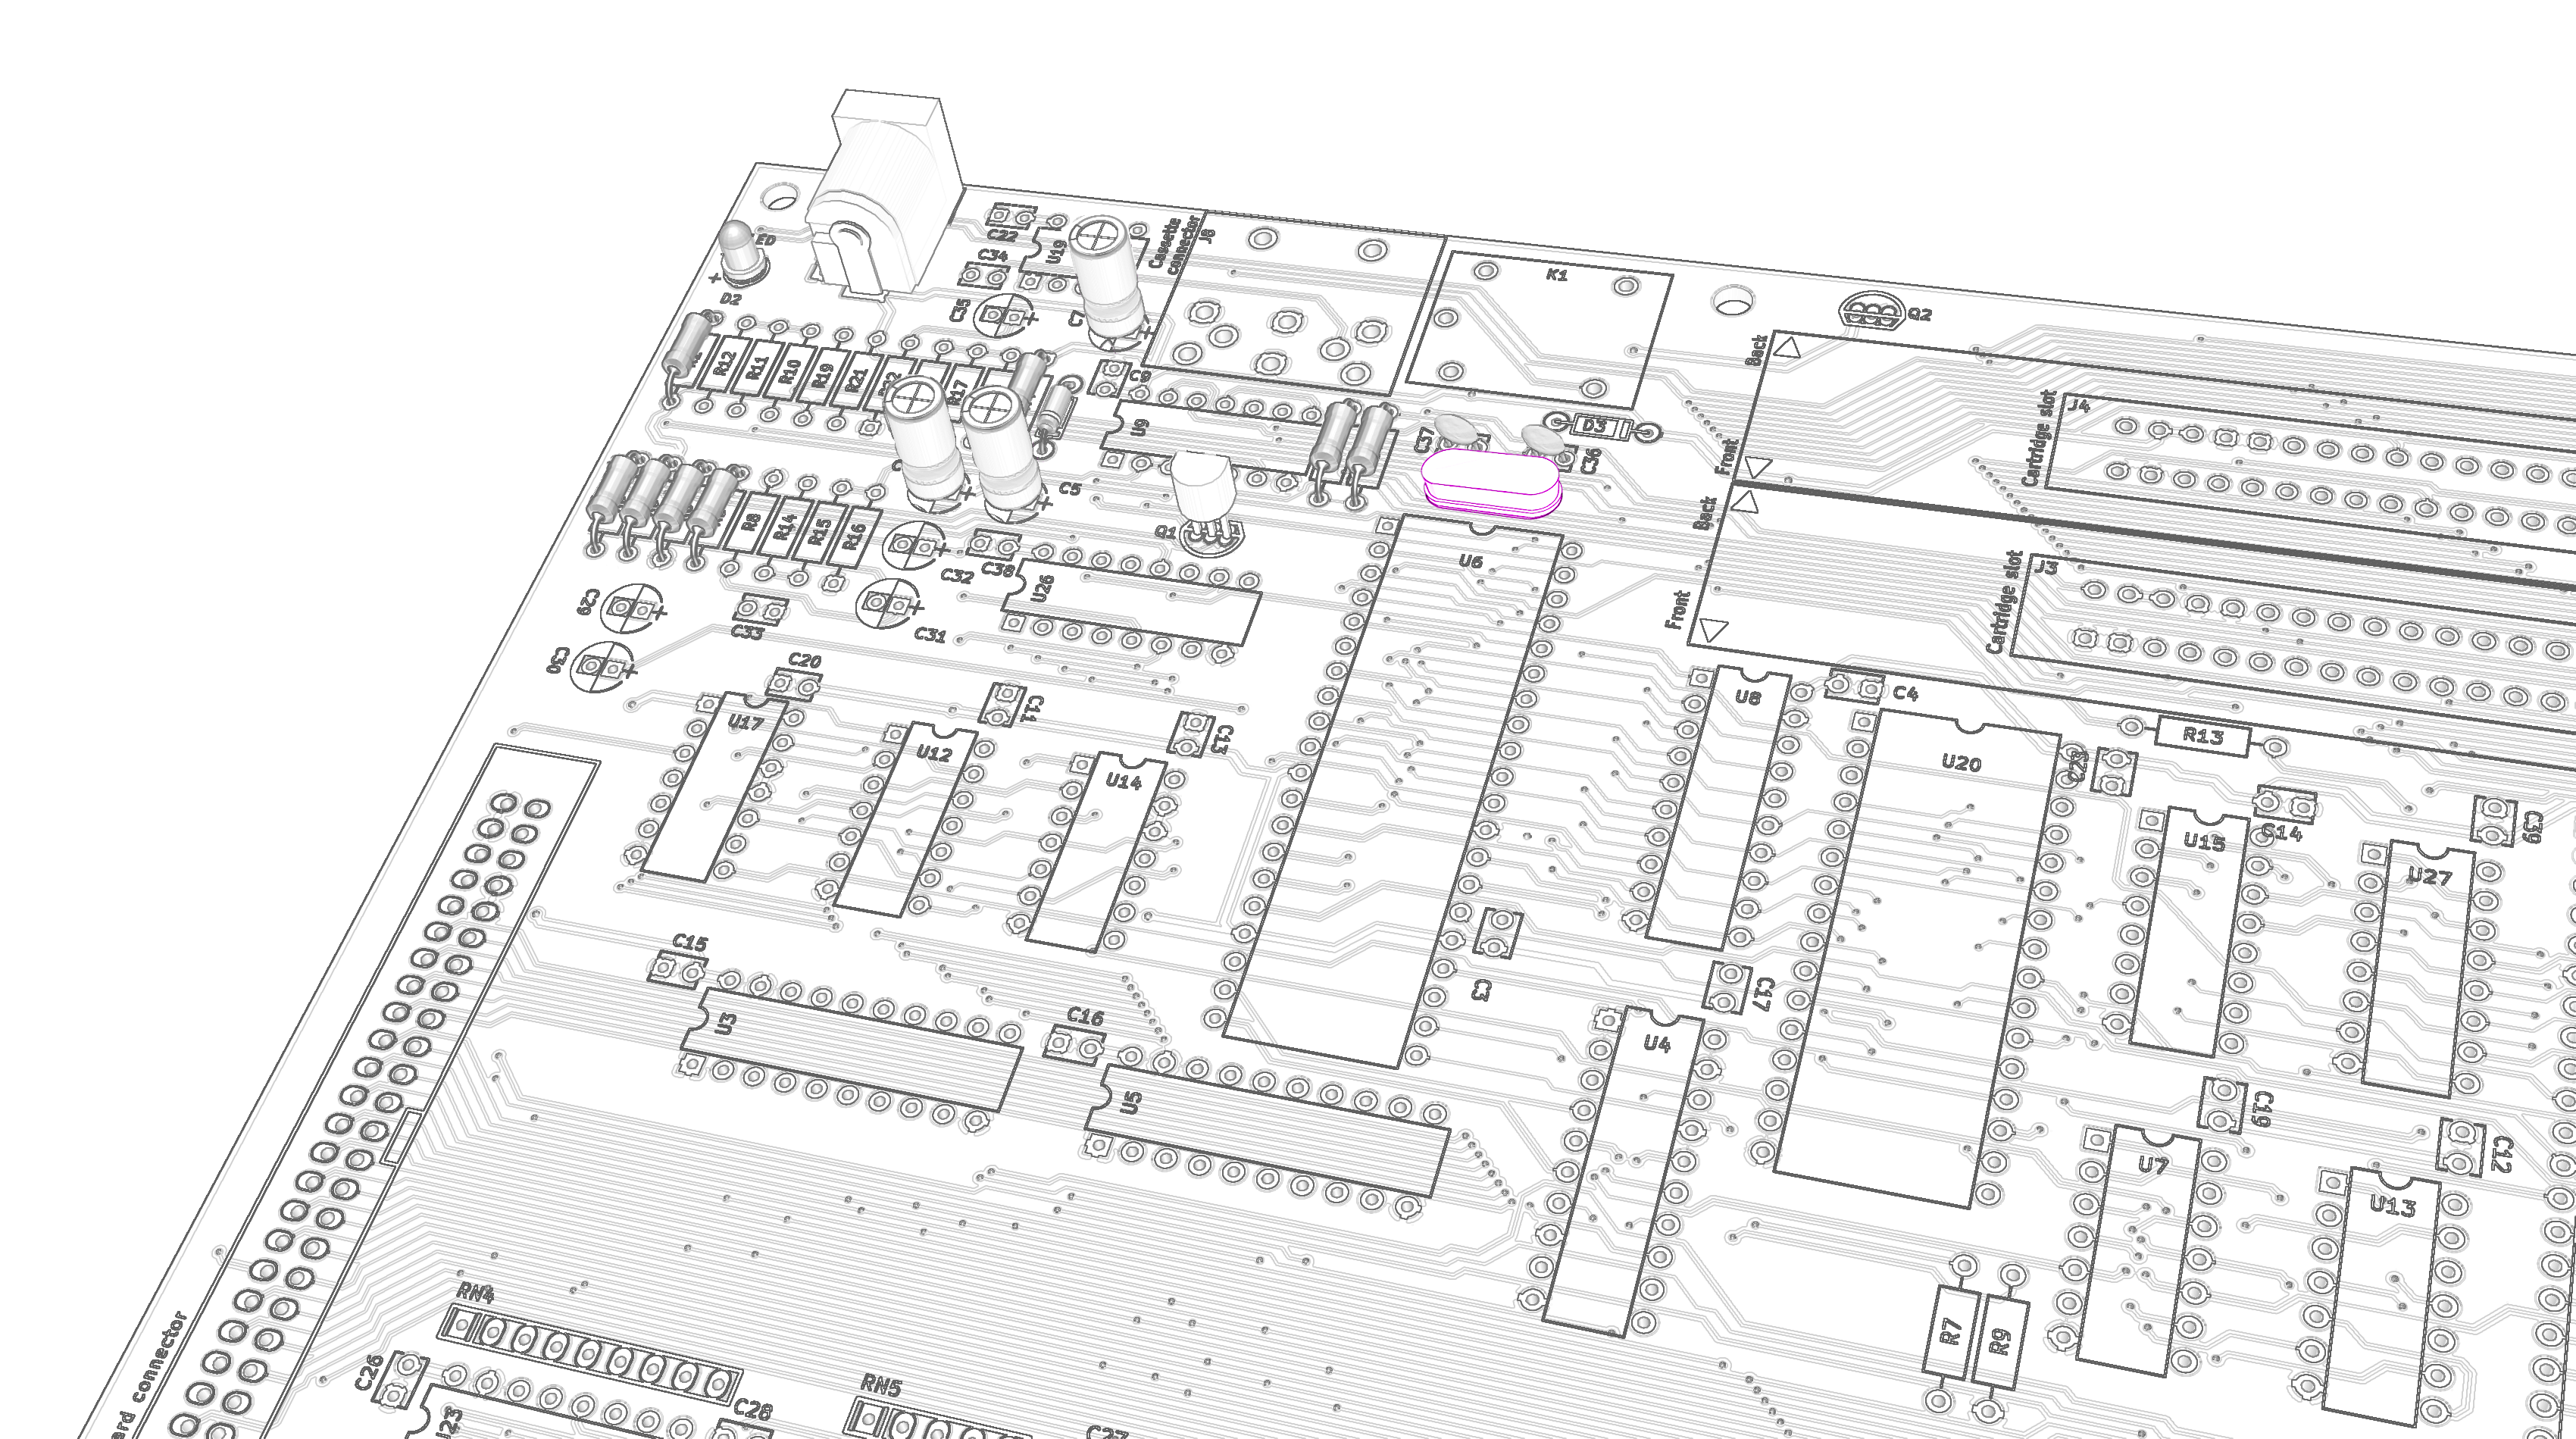
\includegraphics[width=0.8\linewidth]{figures/mount-clock-cpu-03}
  \caption{Placement of quartz crystal {\tt Y1}  of the CPU clock generator}
  \label{fig:mount-clock-cpu-03}
\end{figure}

\begin{figure}[htbp]
  \centering
  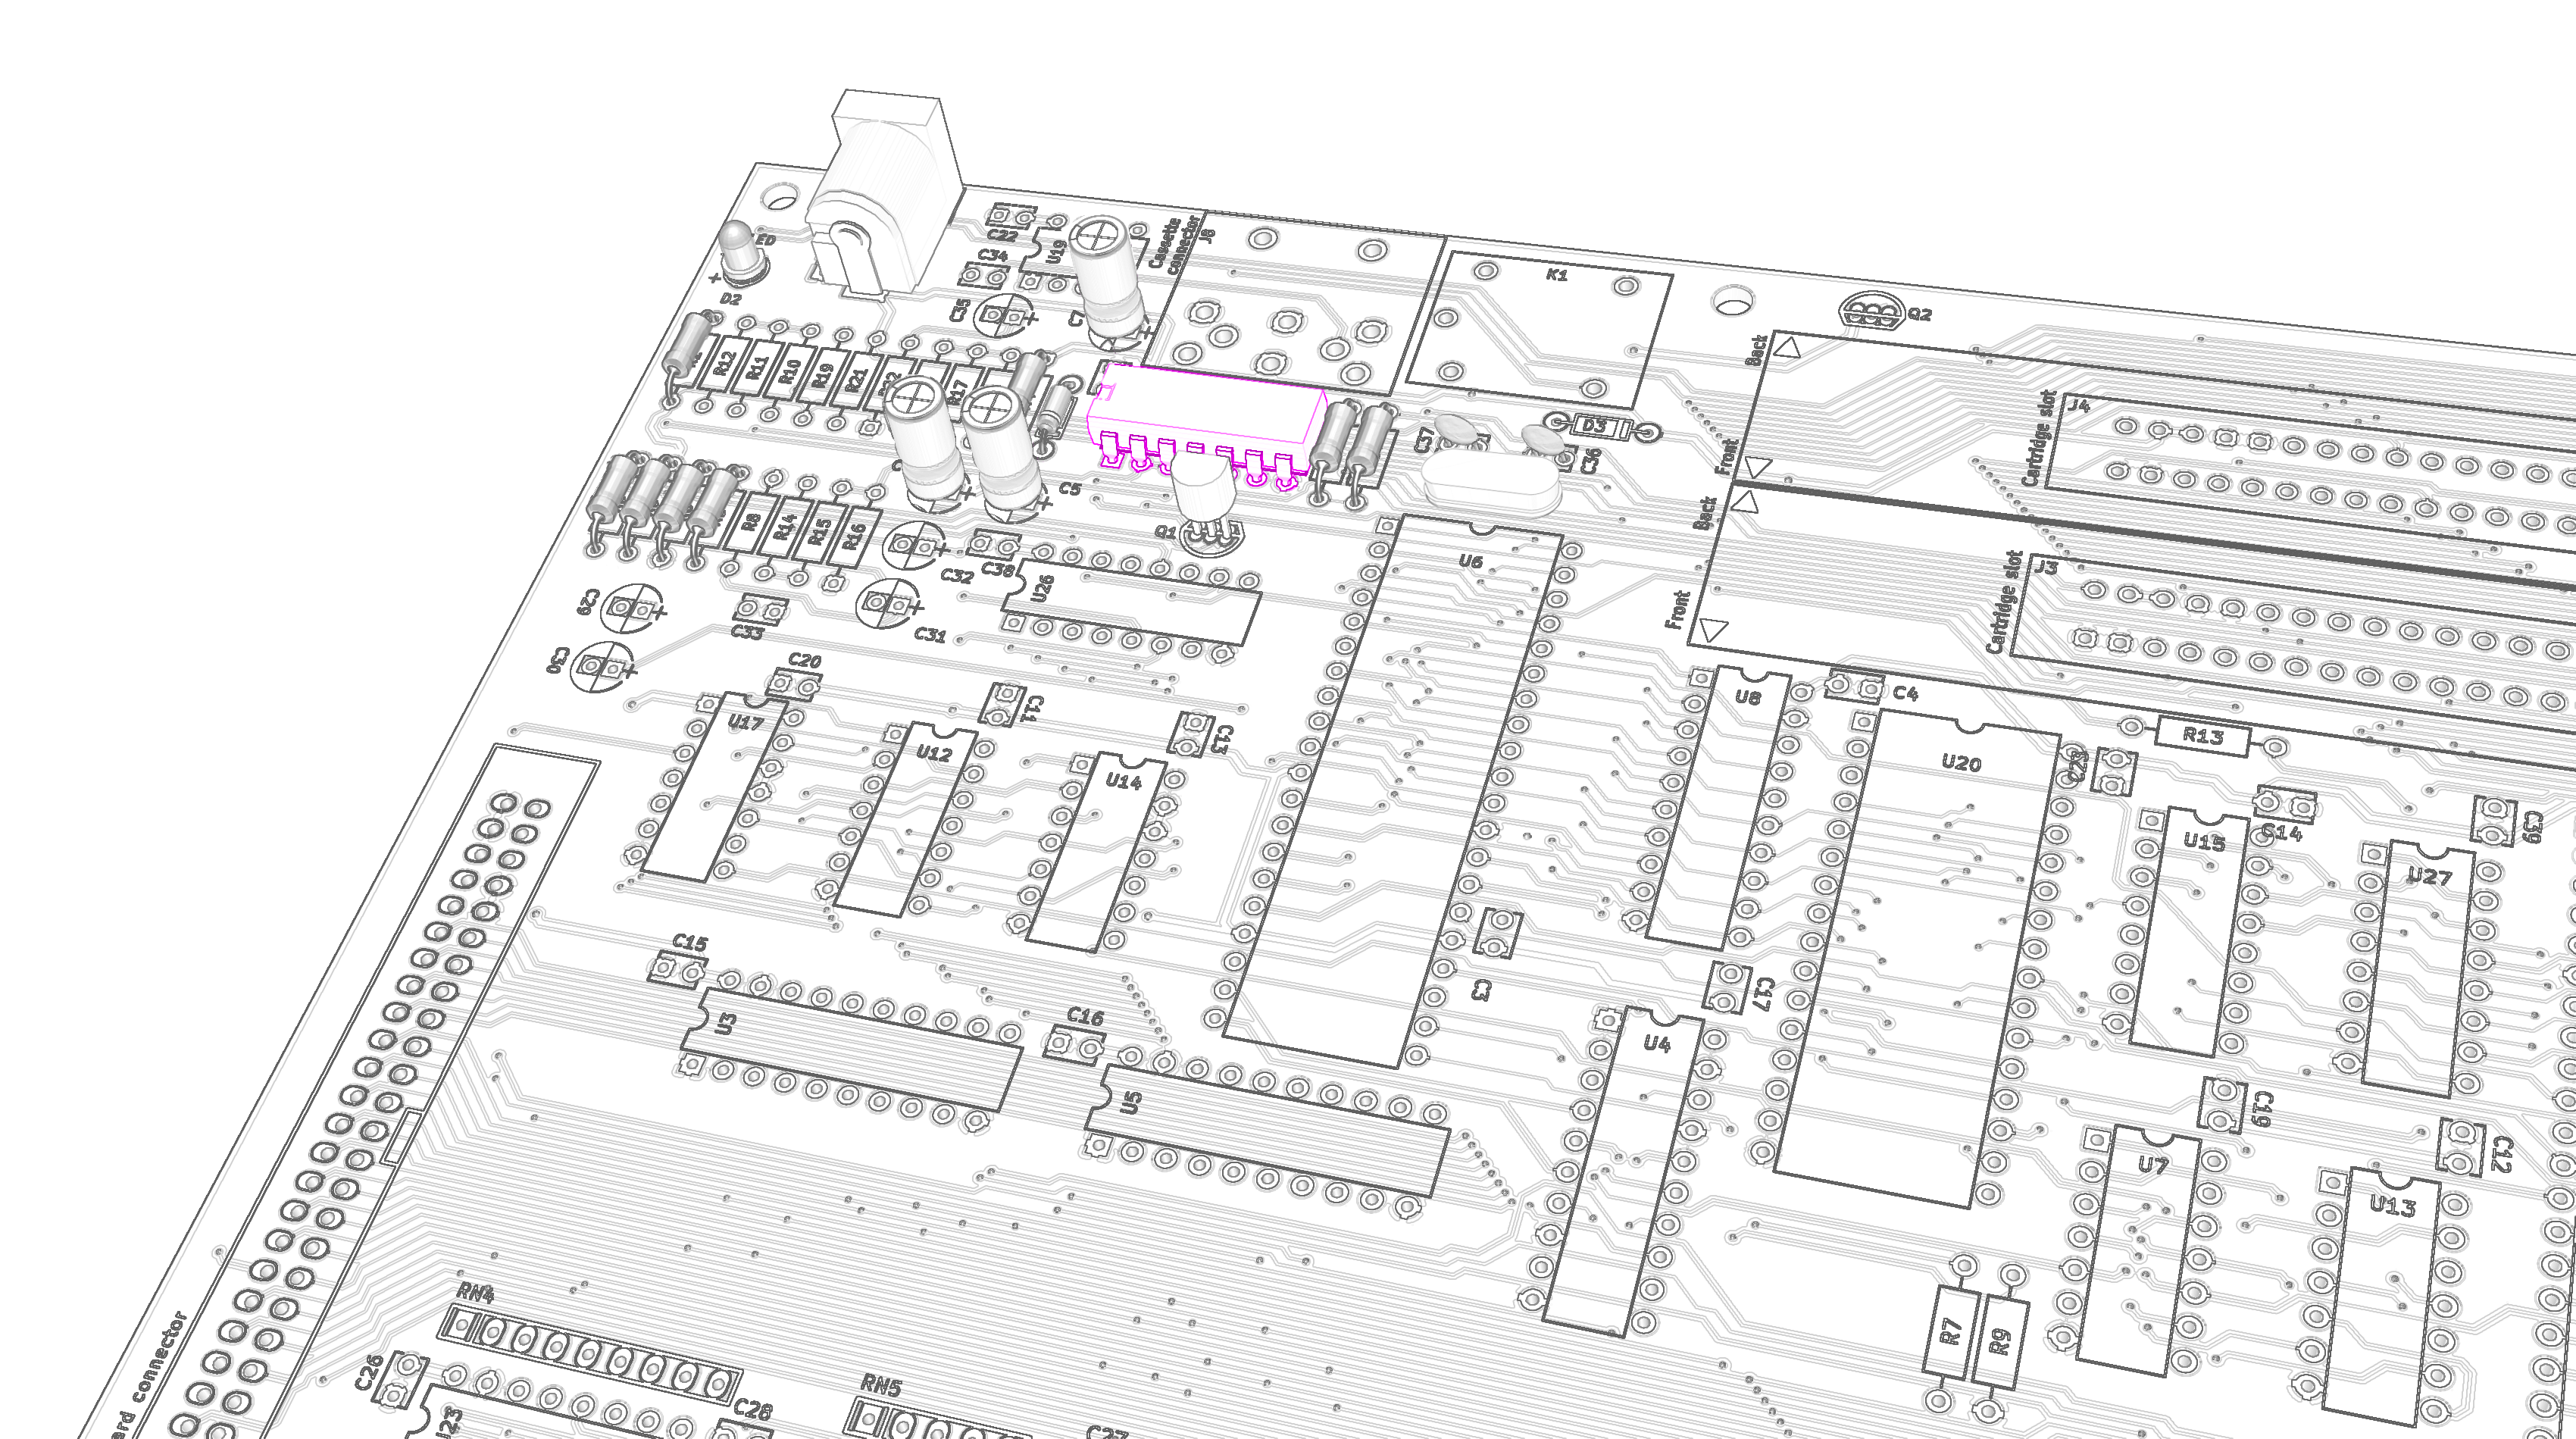
\includegraphics[width=0.8\linewidth]{figures/mount-clock-cpu-04}
  \caption{Placement of logic inverter {\tt U9} of the CPU clock generator}
  \label{fig:mount-clock-cpu-04}
\end{figure}

Once all the parts are assembled, you can perform some tests to check if the CPU clock signal is being generated correctly if you have an oscilloscope at hand. Power on the computer by connecting the power supply to the power jack {\tt J1} and connect your oscilloscope probe to the output of the CMOS inverter {\tt U9F} (pin 12). The oscilloscope should show a square wave with a frequency of 3.58Mhz and a 50\% duty cycle.

If you do not have an oscilloscope, there is nothing to be tested here.

\subsection{PSG clock divider circuit}

After that, we can assemble the elements of the PSG clock divider circuit described in Figure \ref{fig:artemisa-schematic-psg-clock}:

\begin{enumerate}
  \item Solder the decoupling capacitor {\tt C20}, whose placement is shown in Figure \ref{fig:mount-clock-psg-01}.
  \item Solder the D-type flip-flop 74HC74 {\tt U17}, whose placement is shown in Figure \ref{fig:mount-clock-psg-02}.
\end{enumerate}

\begin{figure}[htbp]
  \centering
  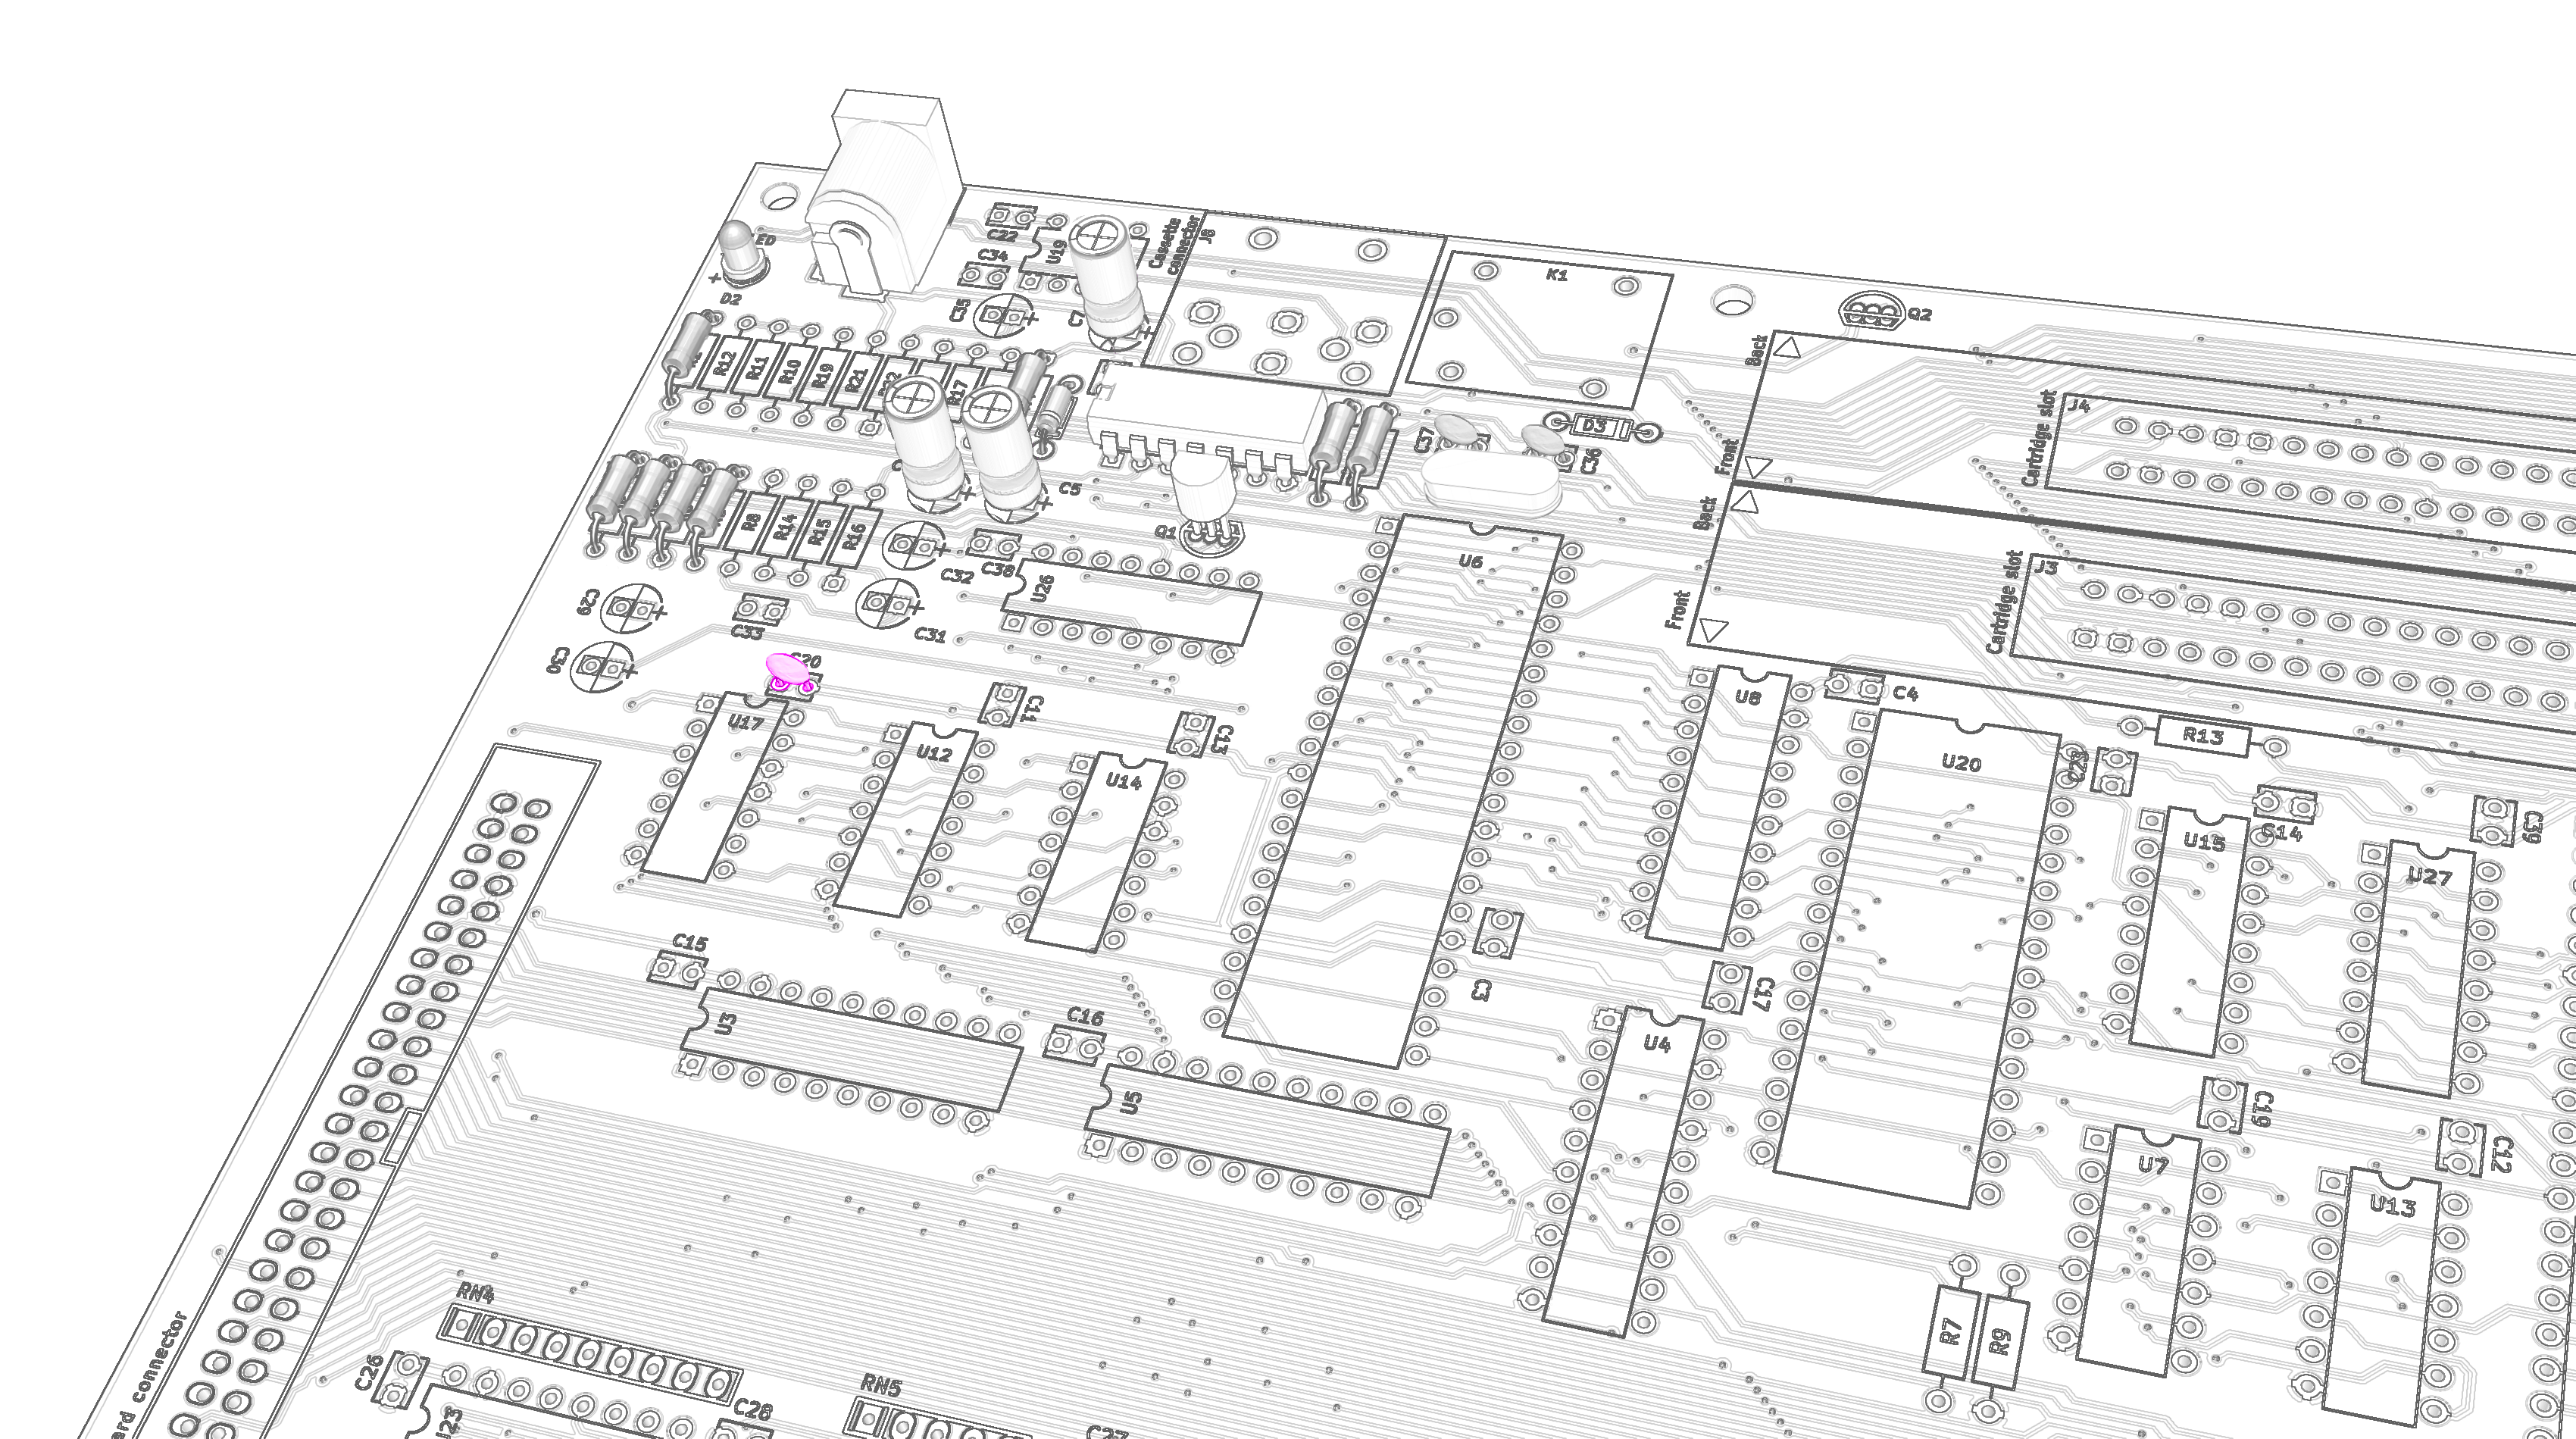
\includegraphics[width=0.8\linewidth]{figures/mount-clock-psg-01}
  \caption{Placement of decoupling capacitor {\tt C20} of the PSG clock divider}
  \label{fig:mount-clock-psg-01}
\end{figure}

\begin{figure}[htbp]
  \centering
  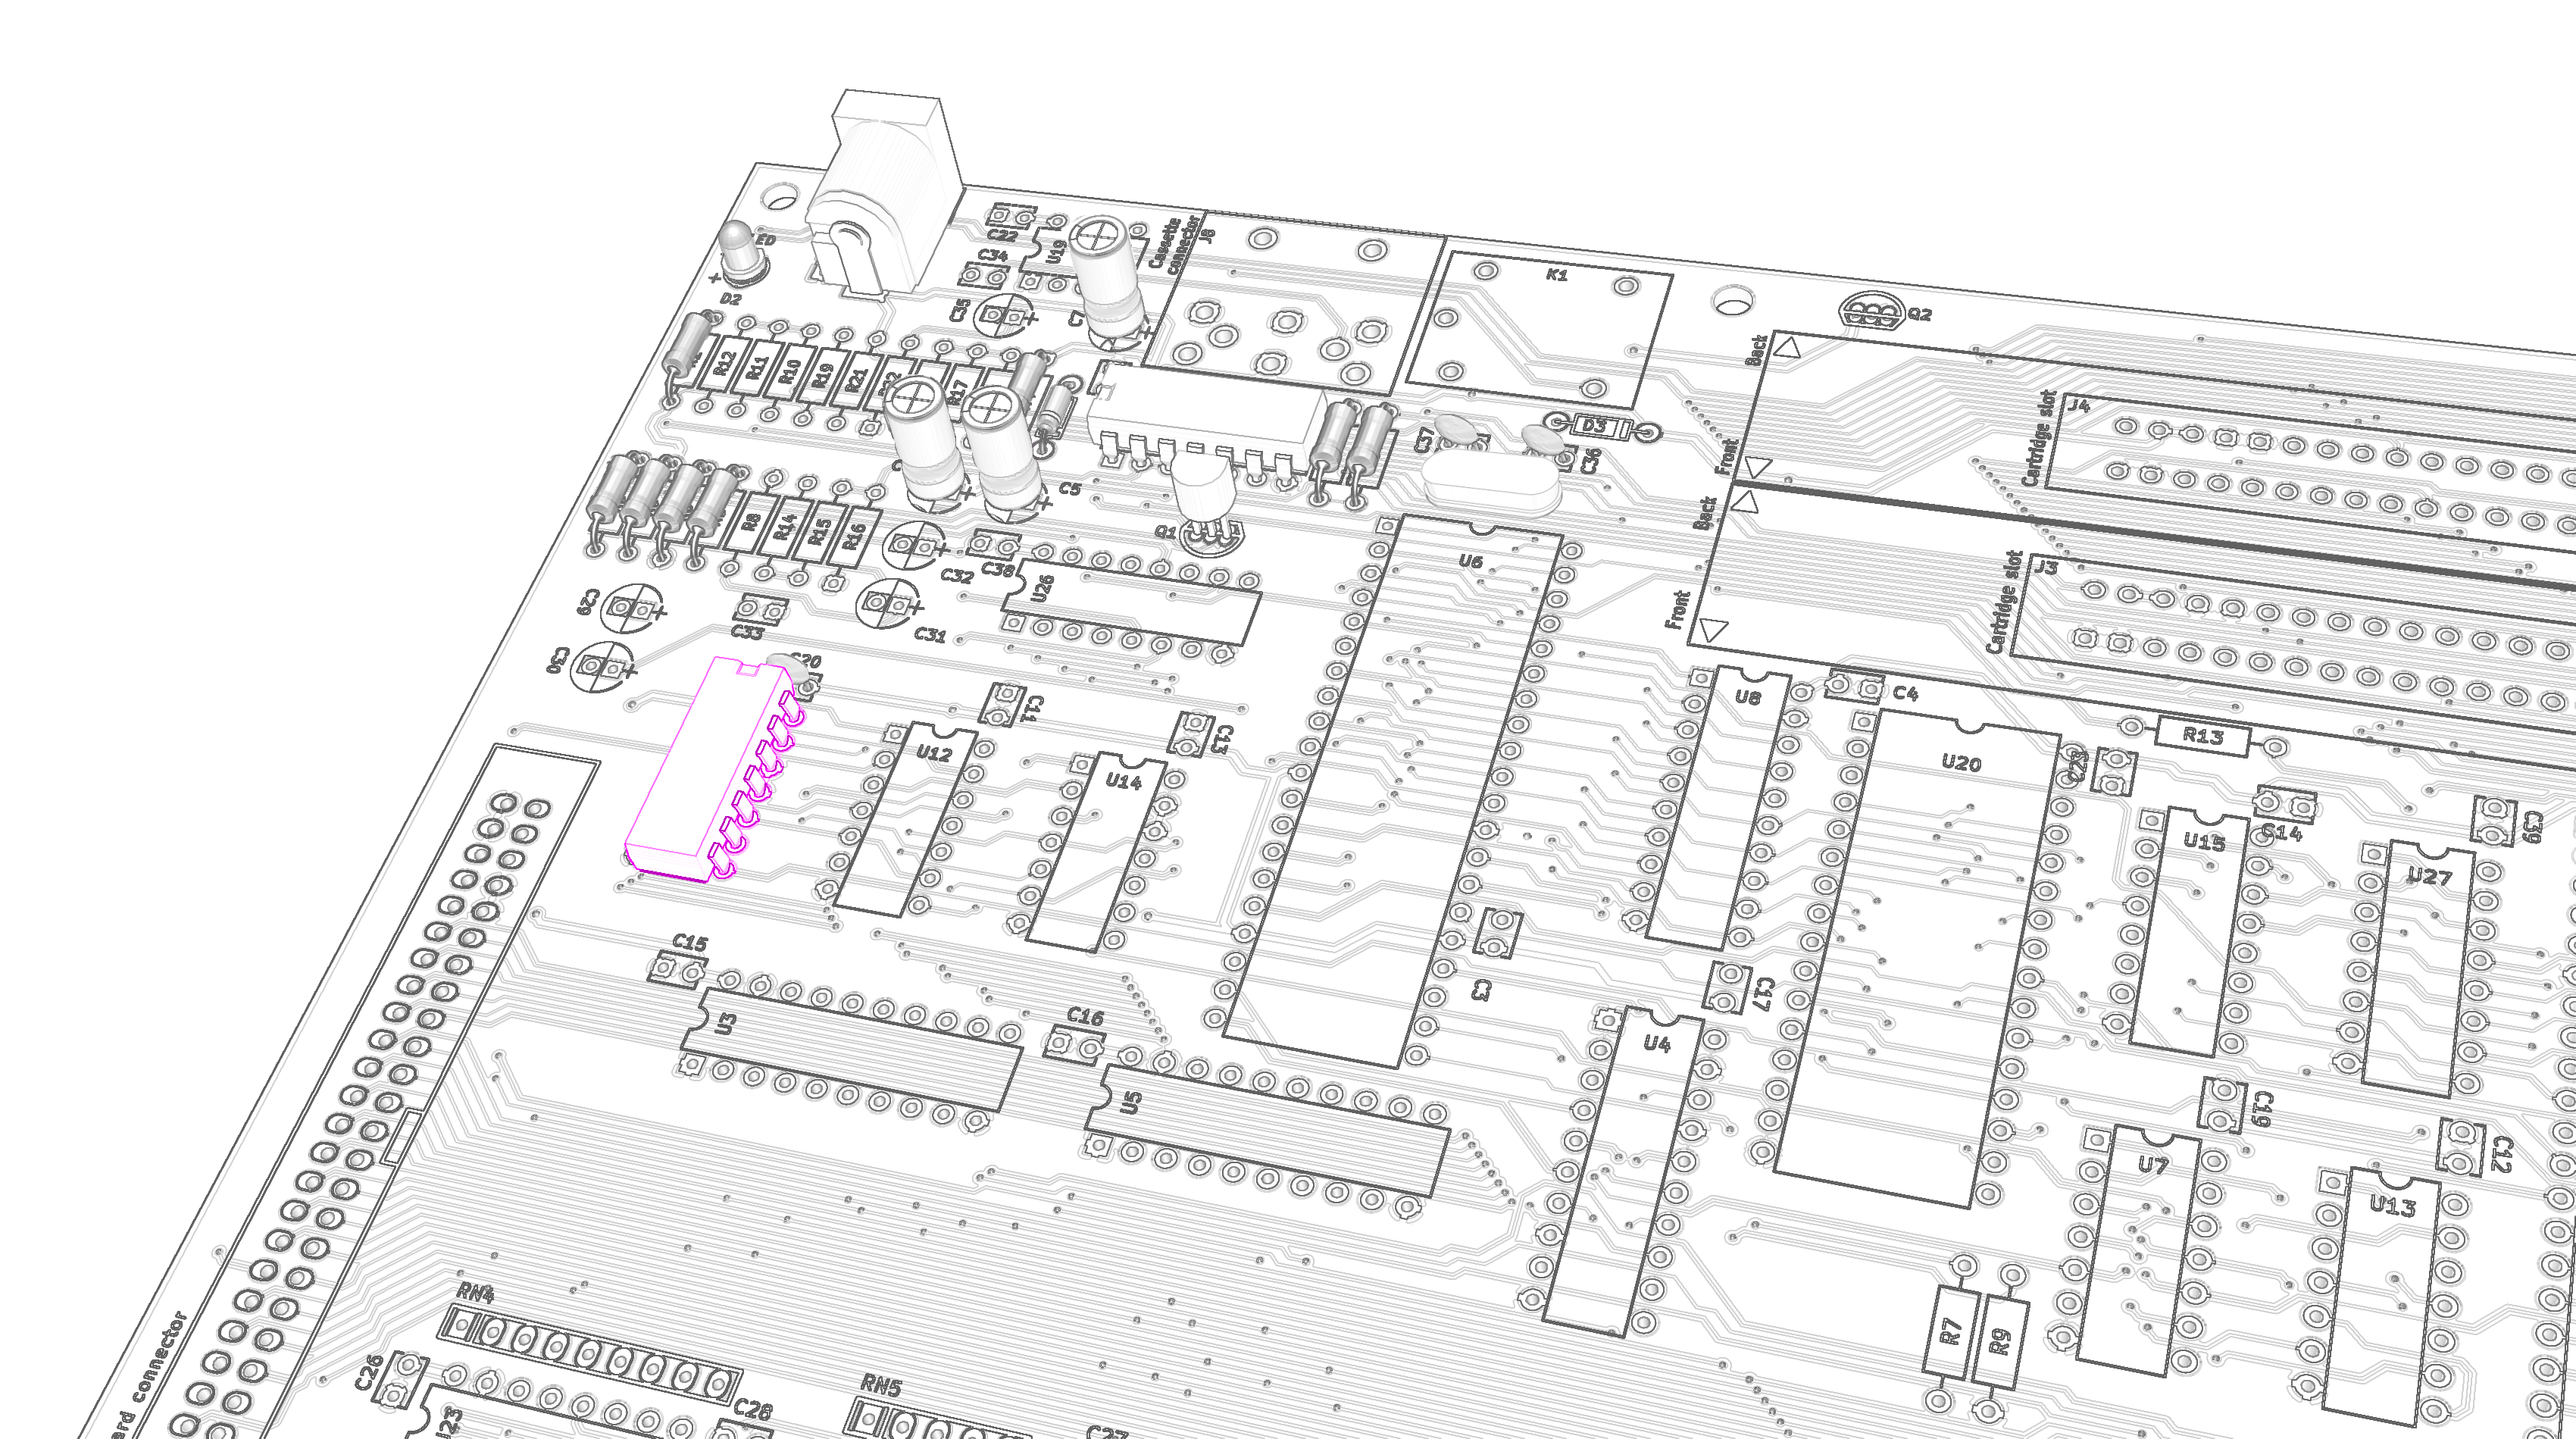
\includegraphics[width=0.8\linewidth]{figures/mount-clock-psg-02}
  \caption{Placement flip-flop 74HC74 of the PSG clock divider}
  \label{fig:mount-clock-psg-02}
\end{figure}

In order to test this part of the circuit, you can use your oscilloscope again. Power the computer on and connect your oscilloscope probe to the output of the flip-flop {\tt U17A} (pin 5). The oscilloscope should show a square wave with a frequency of 1.79Mhz and a 50\% duty cycle.

If you do not have an oscilloscope, there is nothing to be tested here.
